% \documentclass[aspectratio=169,notes]{beamer}
\documentclass[aspectratio=169]{beamer}
\usetheme[faculty=phil]{fibeamer}
\usepackage{polyglossia}
\setmainlanguage{english} %% main locale instead of `english`, you
%% can typeset the presentation in either Czech or Slovak,
%% respectively.
\setotherlanguages{russian} %% The additional keys allow
%%
%%   \begin{otherlanguage}{czech}   ... \end{otherlanguage}
%%   \begin{otherlanguage}{slovak}  ... \end{otherlanguage}
%%
%% These macros specify information about the presentation
\title[Introduction to Robotics (In2Ro)]{Introduction to Robotics, Lecture 8} %% that will be typeset on the
\subtitle{Wheel constraints and holonomy
\\ Polar feedback control \\ Global and local navigation  } %% title page.
\author{Oleg Bulichev}
%% These additional packages are used within the document:
\usepackage{ragged2e}  % `\justifying` text
\usepackage{booktabs}  % Tables
\usepackage{tabularx}
\usepackage{tikz}      % Diagrams
\usetikzlibrary{calc, shapes, backgrounds, trees, positioning, arrows.meta}
\usetikzlibrary{decorations.pathreplacing,calligraphy,calc,graphs}
\usepackage{amsmath, amssymb}
\usepackage{url}       % `\url`s
\usepackage{listings}  % Code listings
\usepackage{floatrow}
\usepackage{subcaption}
\usepackage{mathtools}
\usepackage{todonotes}
\usepackage{fontspec}
\usepackage{multicol}
\usepackage{pdfpages}
\usepackage{wrapfig}
\usepackage{qrcode}
\usepackage{animate}
\usepackage{booktabs}
\usepackage{multirow}
\usepackage{graphicx}
\usepackage{colortbl}

\graphicspath{{resources/}}
\frenchspacing

\setbeamertemplate{caption}{\raggedright\insertcaption\par}
\usetikzlibrary{graphs}

% \usepackage[backend=biber,style=ieee,autocite=footnote]{biblatex}
% \addbibresource{biblio.bib}
% \DefineBibliographyStrings{english}{%
%   bibliography = {References},}

\newcommand{\oleg}[2][] {\todo[color=red, #1] {OLEG:\\ #2}}
\newcommand{\fbckg}[1]{\usebackgroundtemplate{\includegraphics[width=\paperwidth]{#1}}}%frame background

\usepackage[framemethod=TikZ]{mdframed}
\newcommand{\dbox}[1]{
\begin{mdframed}[roundcorner=3pt, backgroundcolor=yellow, linewidth=0]
\vspace{1mm}
{#1}
\vspace{1mm}
\end{mdframed}
}

\begin{document}
\setlength{\abovedisplayskip}{0pt}
\setlength{\belowdisplayskip}{0pt}
\setlength{\abovedisplayshortskip}{0pt}
\setlength{\belowdisplayshortskip}{0pt}

\fbckg{fibeamer/figs/title_page.png}
\frame[c]{\setcounter{framenumber}{0}
    \usebeamerfont{title}%
    \usebeamercolor[fg]{title}%
    \begin{minipage}[b][6.5\baselineskip][b]{\textwidth}%
        \textcolor{black}{\raggedright\inserttitle}
    \end{minipage}
    % \vskip-1.5\baselineskip

    \usebeamerfont{subtitle}%
    \usebeamercolor[fg]{framesubtitle}%
    \begin{minipage}[b][3\baselineskip][b]{\textwidth}
        \raggedright%
        \insertsubtitle%
    \end{minipage}
    \vskip.25\baselineskip
}

\fbckg{fibeamer/figs/common.png}

\begin{frame}[t]{Where we stopped, and why we go back}
\small
\setlength{\abovedisplayskip}{1mm}\setlength{\belowdisplayskip}{1mm}
\setlength{\abovedisplayshortskip}{0pt}\setlength{\belowdisplayshortskip}{0pt}
\begin{block}{From one wheel to a useful base}
W07 ended at manoeuvrability. We revisit the constraints slowly, using differential drive, three-Swedish omni, and differential drive with a castor.
\end{block}\vspace{2mm}
\begin{block}{Three properties to read}
A \textbf{constraint} forbids a motion. \textbf{Mobility} counts independent instantaneous velocities. \textbf{Steerability} counts independent steering changes.
\end{block}\vspace{2mm}
An \textbf{instantaneous centre of rotation (ICR)} is the point about which the chassis turns at an instant. One wheel-by-wheel recipe lets us compare the bases.
\end{frame}

\begin{frame}[t]{One method: constrain each wheel, then stack}
\small
\setlength{\abovedisplayskip}{1mm}\setlength{\belowdisplayskip}{1mm}
\setlength{\abovedisplayshortskip}{0pt}\setlength{\belowdisplayshortskip}{0pt}
\begin{columns}[T,onlytextwidth]\begin{column}{0.49\textwidth}
\begin{block}{1. Constrain each wheel}
Rolling: speed along its driven direction matches wheel spin. Sliding: no speed across a standard wheel.
\end{block}\vspace{2mm}
\begin{block}{2. Stack the rows}
\[J_1(\beta_s)\dot\xi_R=J_2\dot\varphi,\qquad C_1(\beta_s)\dot\xi_R=0.\]
\end{block}\vspace{2mm}
\end{column}\begin{column}{0.49\textwidth}
\begin{block}{Read the symbols}
$\xi=(x,y,\theta)^T$: planar pose. $\dot\xi_R=(\dot x_R,\dot y_R,\dot\theta)^T$: velocity in the robot coordinate frame. $\dot\xi_R=R(\theta)\dot\xi_I$, where $R$ maps global velocities to robot coordinates. $\dot\varphi$: wheel spin rates. $\beta_s$: steerable-wheel angles.
\end{block}\vspace{2mm}
\begin{block}{3. Read the mobility}
$J_1$: rolling rows; $J_2$: wheel-radius factors; $C_1$: sliding rows. Rank counts independent forbidden directions. $\delta_m=3-\operatorname{rank}C_1$ is mobility.
\end{block}\vspace{2mm}
\end{column}\end{columns}
\end{frame}

\begin{frame}[t]{A fixed wheel allows rolling and forbids sliding}
\small
\setlength{\abovedisplayskip}{1mm}\setlength{\belowdisplayskip}{1mm}
\setlength{\abovedisplayshortskip}{0pt}\setlength{\belowdisplayshortskip}{0pt}
\begin{columns}[T,onlytextwidth]\begin{column}{0.49\textwidth}\centering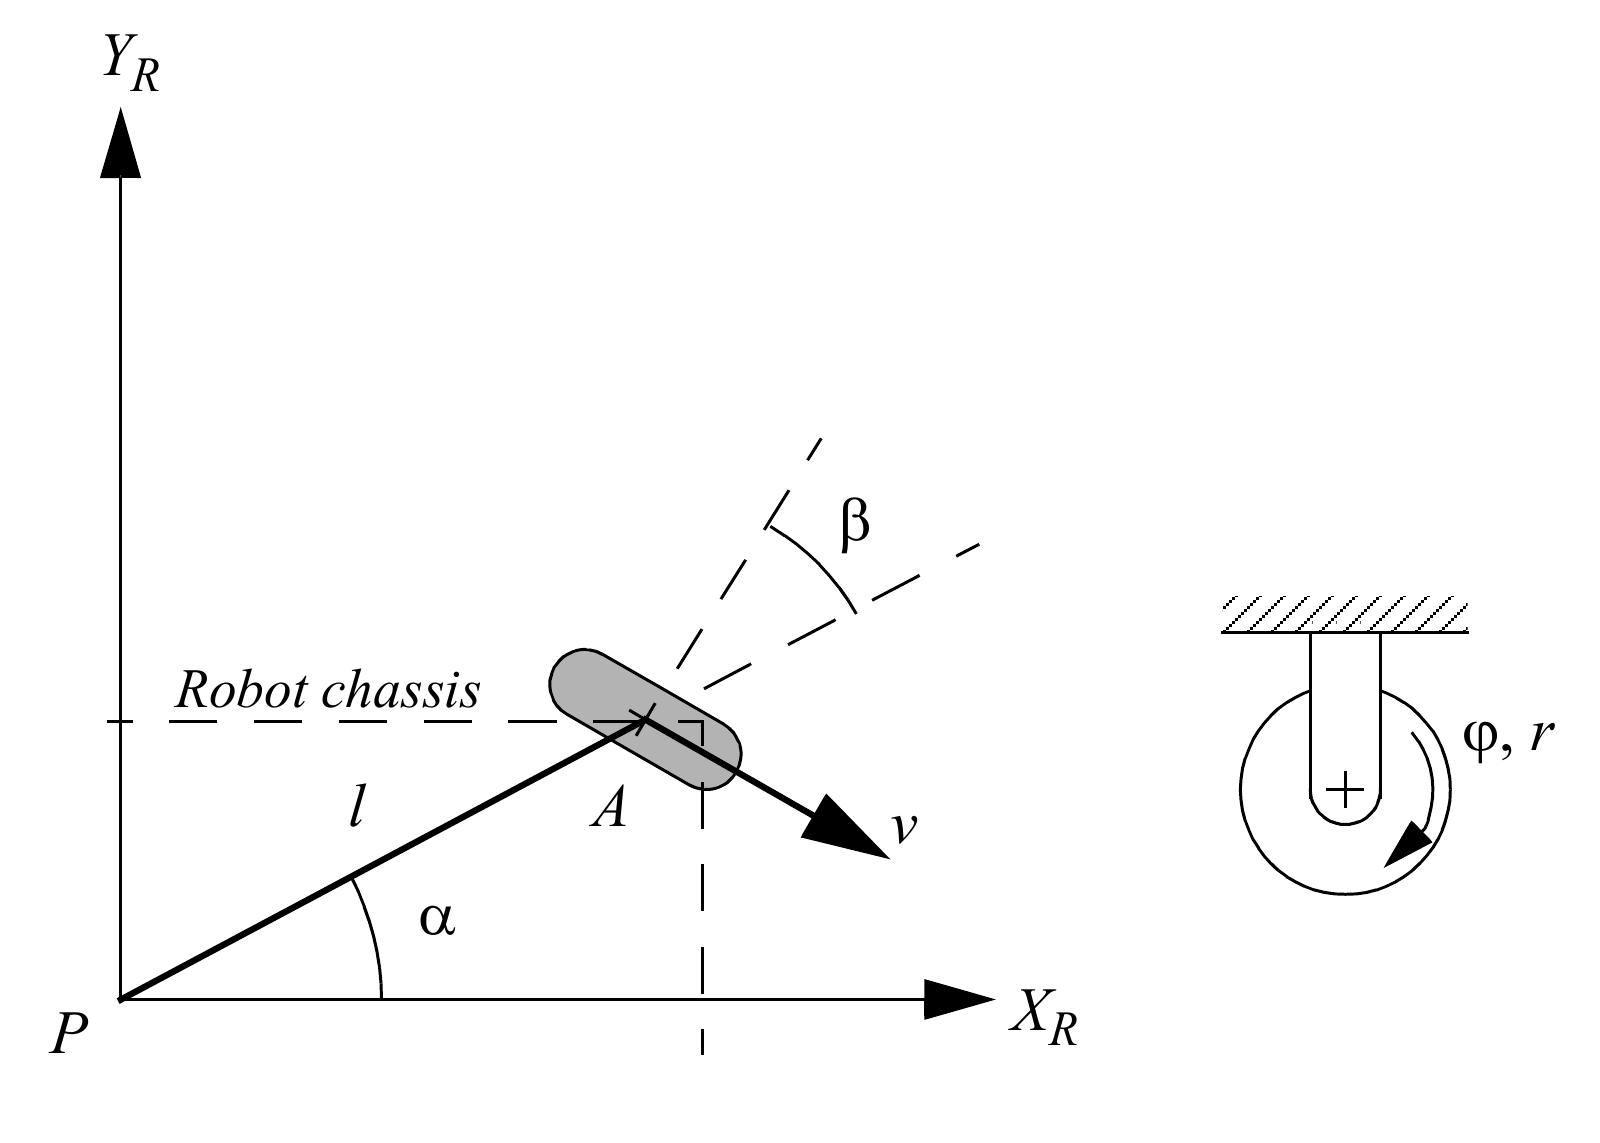
\includegraphics[width=\linewidth,height=4.5cm,keepaspectratio]{book_p081.png}\par\raggedright $l$: centre-to-wheel distance; $\alpha$: polar position angle; $\beta$: plane orientation; $r$: radius; $\varphi$: spin angle.\end{column}\begin{column}{0.49\textwidth}\textbf{Rolling without slip}\[\begin{aligned}\sin(\alpha+\beta)\dot x_R&-\cos(\alpha+\beta)\dot y_R\\&-l\cos\beta\,\dot\theta=r\dot\varphi.\end{aligned}\]Contact speed along the wheel plane matches rim speed.\vspace{3mm}\par\textbf{No sideways sliding}\[\begin{aligned}\cos(\alpha+\beta)\dot x_R&+\sin(\alpha+\beta)\dot y_R\\&+l\sin\beta\,\dot\theta=0.\end{aligned}\]Contact speed across the plane is zero.\end{column}\end{columns}
\end{frame}

\begin{frame}[t]{Worked example: one fixed wheel}
\small
\setlength{\abovedisplayskip}{1mm}\setlength{\belowdisplayskip}{1mm}
\setlength{\abovedisplayshortskip}{0pt}\setlength{\belowdisplayshortskip}{0pt}
\begin{block}{Substitute the geometry}
$\alpha=90^\circ$, $\beta=0$, $l=0.2$ m, $r=0.05$ m, $\theta=0$. Global and robot coordinates coincide.\[\underbrace{[1\quad0\quad-l]\dot\xi_R=r\dot\varphi}_{\text{rolling}}\qquad\underbrace{[0\quad1\quad0]\dot\xi_R=0}_{\text{sliding}}\]
\end{block}\vspace{2mm}
\begin{block}{The two measurable statements}
\[\dot x_R-0.2\dot\theta=0.05\dot\varphi,\qquad\dot y_R=0.\] If $\dot\varphi=10$ rad/s and $\dot\theta=0$, the robot moves forward at $0.5$ m/s and cannot move sideways.
\end{block}\vspace{2mm}

\end{frame}

\begin{frame}[t]{Steered wheel and castor wheel}
\small
\setlength{\abovedisplayskip}{1mm}\setlength{\belowdisplayskip}{1mm}\setlength{\abovedisplayshortskip}{0pt}\setlength{\belowdisplayshortskip}{0pt}
\begin{columns}[T,onlytextwidth]\begin{column}{.49\textwidth}{\centering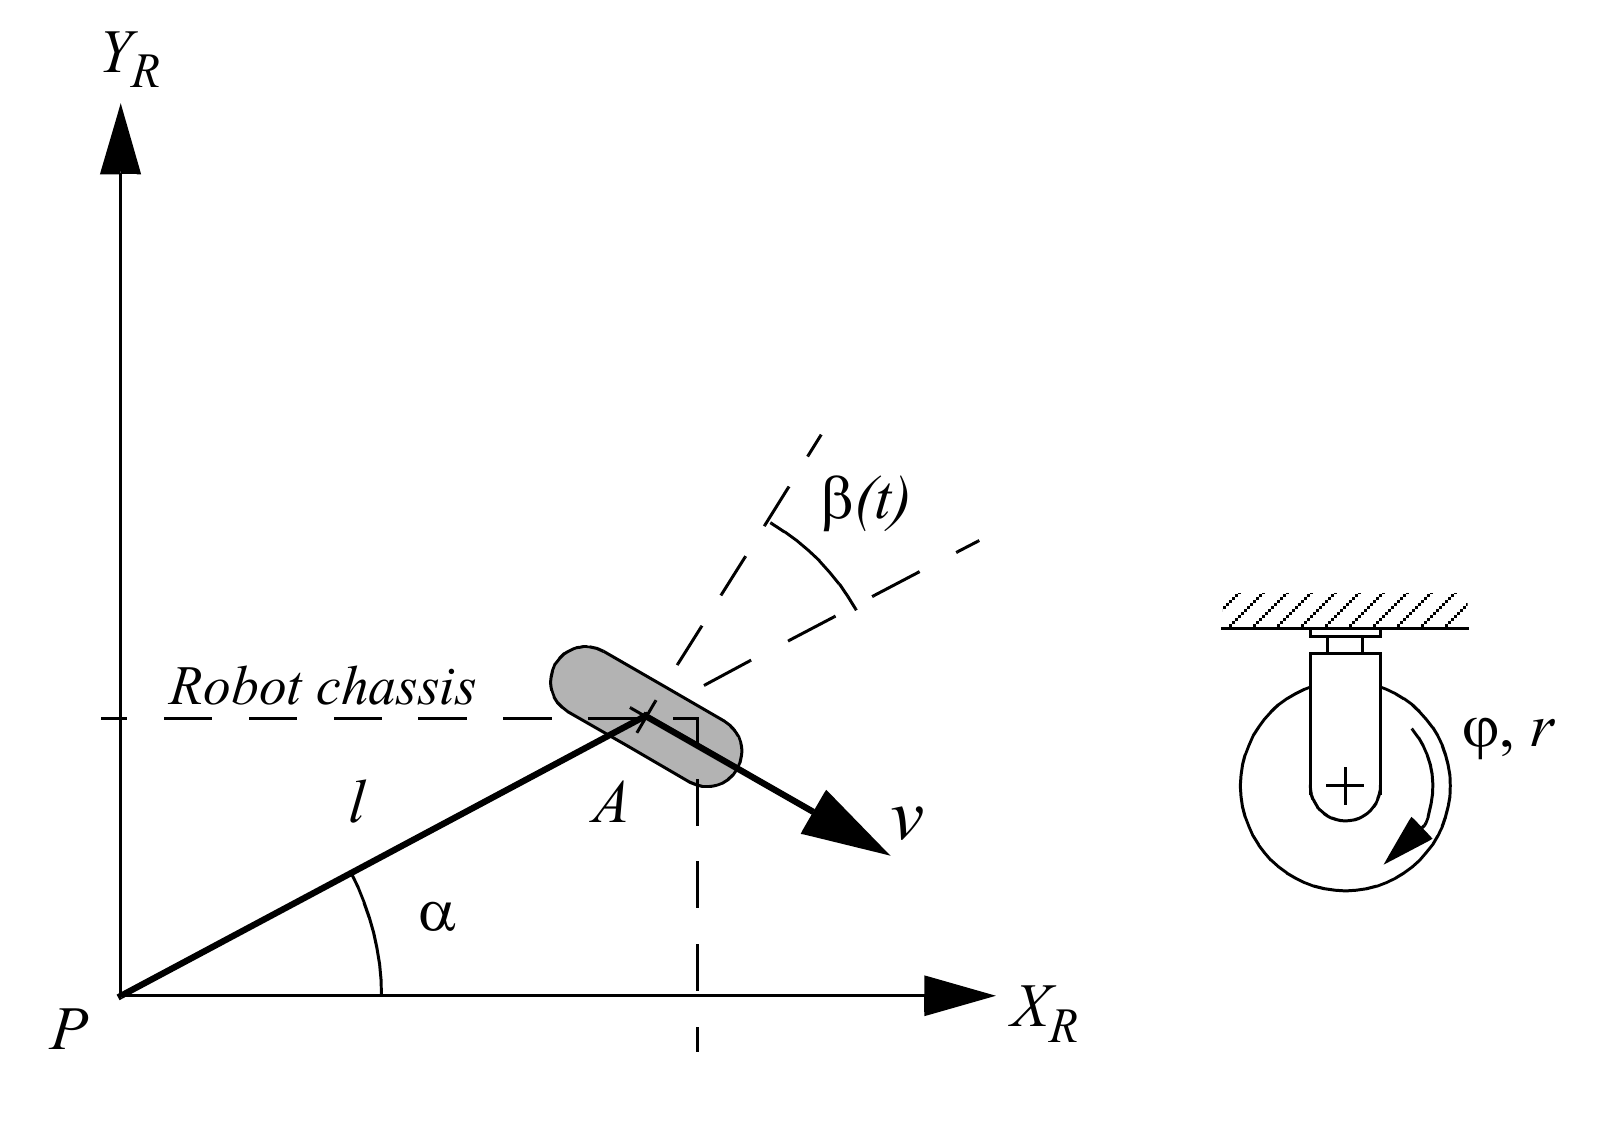
\includegraphics[width=\linewidth,height=5.5cm,keepaspectratio]{book_p083.png}\par}\textbf{Steered}: choose $\beta(t)$, the wheel-plane angle. Same rolling/sliding rows.\end{column}\begin{column}{.49\textwidth}{\centering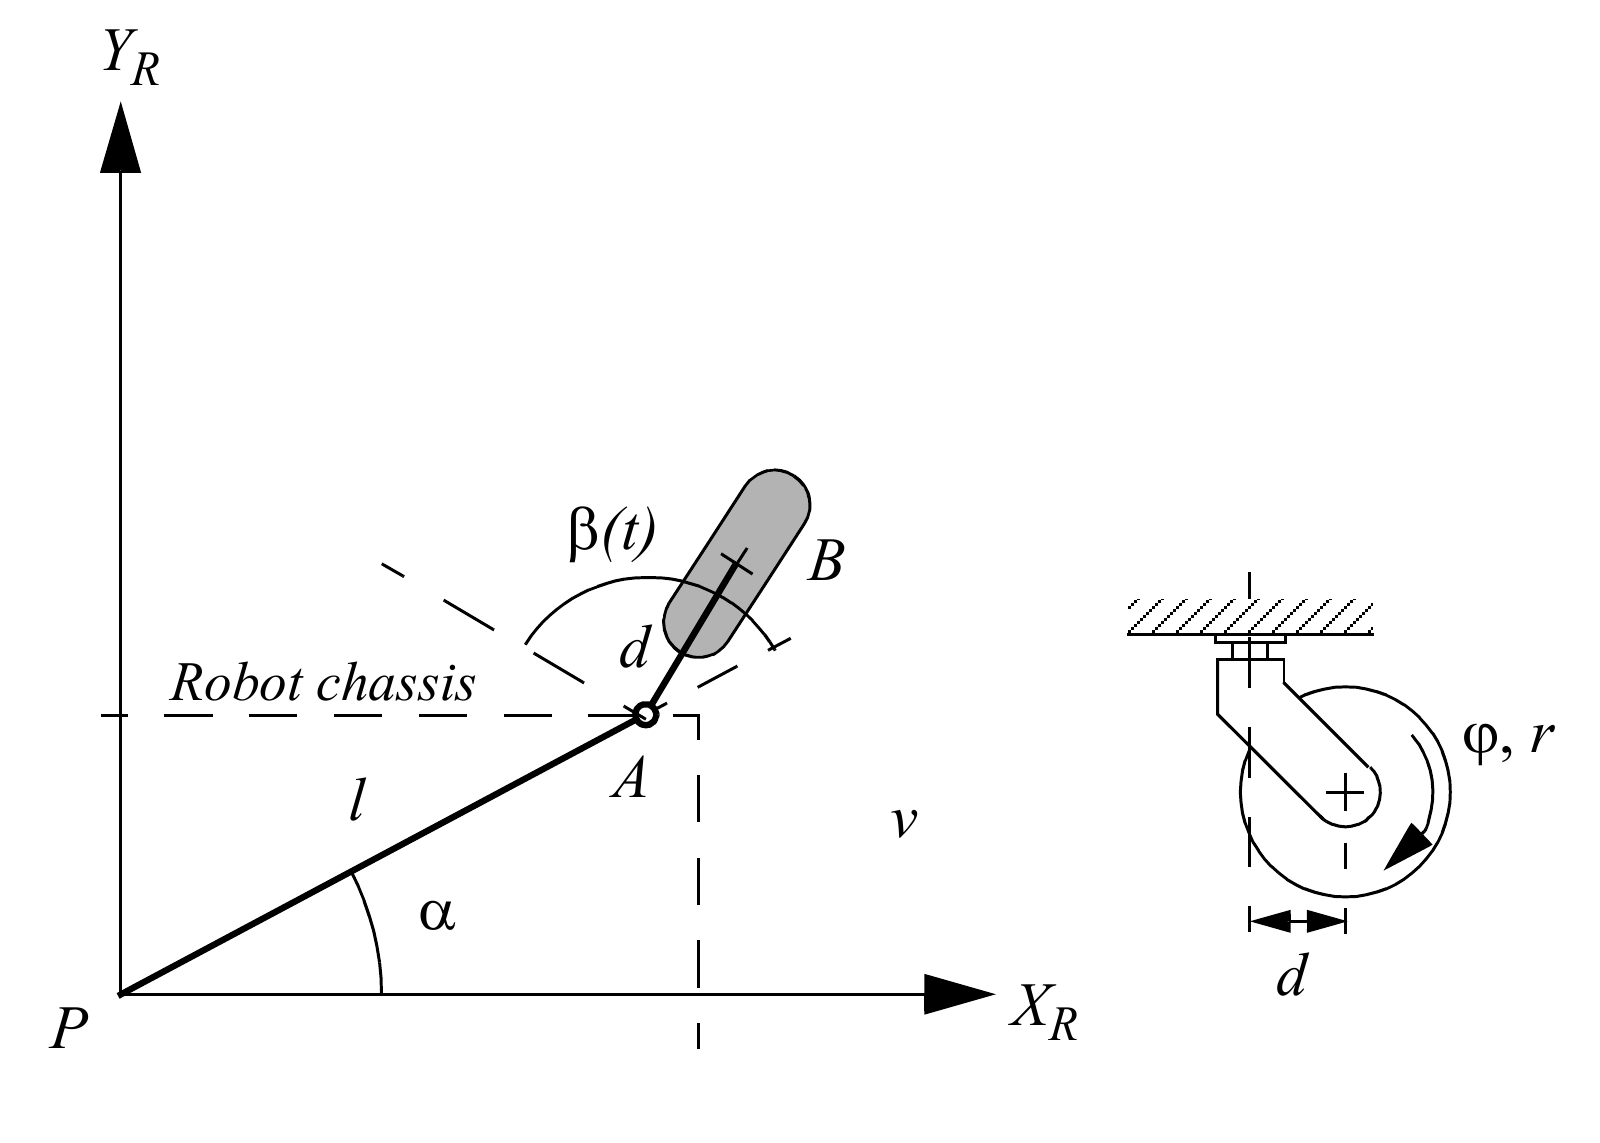
\includegraphics[width=\linewidth,height=5.5cm,keepaspectratio]{book_p084.png}\par}\textbf{Castor}: offset $d$ adds $d\dot\beta$. Free pivot: no chassis constraint, only support.\end{column}\end{columns}
\end{frame}

\begin{frame}[t]{Swedish wheel: rollers remove the sliding constraint}
\small
\setlength{\abovedisplayskip}{1mm}\setlength{\belowdisplayskip}{1mm}
\begin{columns}[T,onlytextwidth]\begin{column}{0.49\textwidth}{\centering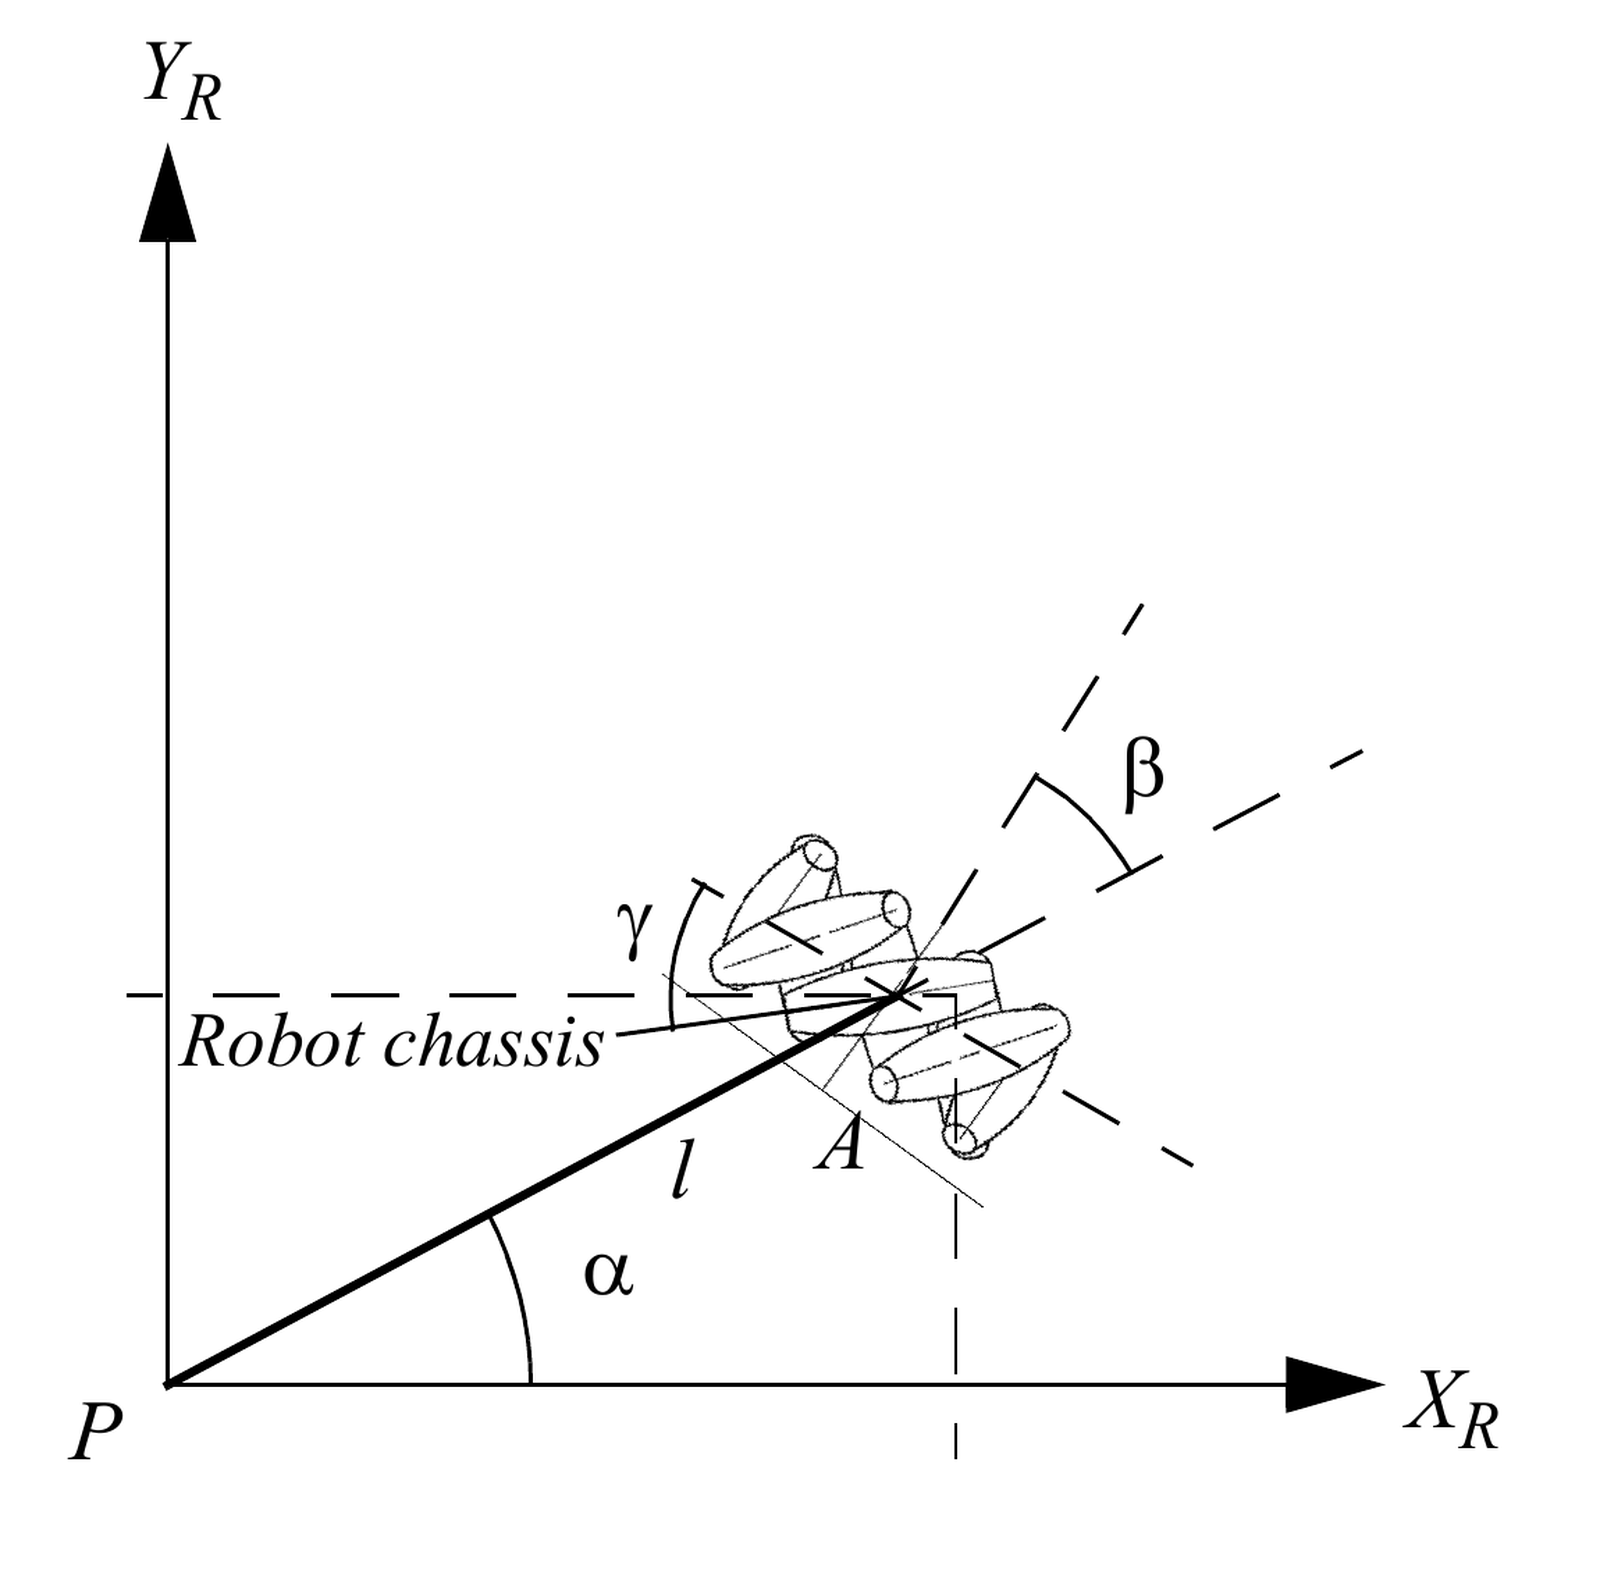
\includegraphics[width=\linewidth,height=4.5cm,keepaspectratio]{book_p086.png}\par}\end{column}\begin{column}{0.49\textwidth}A \textbf{roller} is a freely spinning small rim wheel. $\gamma$ is the angle between its axis and the main wheel plane. Roller spin leaves one contact direction free.\par\vspace{3mm}$\gamma=0$: Swedish $90^\circ$ wheel. The standard rolling row remains; no lateral sliding row. Driven and free directions decouple.\par\vspace{3mm}$\gamma=\pi/2$: degenerate and excluded. Lateral constraint remains, rolling constraint disappears; main-wheel spin is unnecessary.\end{column}\end{columns}
\end{frame}

\begin{frame}[t]{Stacking: J1, J2 and C1}
\small
\setlength{\abovedisplayskip}{1mm}\setlength{\belowdisplayskip}{1mm}

\setlength{\abovedisplayskip}{1mm}\setlength{\belowdisplayskip}{1mm}
\setlength{\abovedisplayshortskip}{0pt}\setlength{\belowdisplayshortskip}{0pt}
\begin{block}{Rolling rows collect the wheel speeds}
\[J_1(\beta_s)\dot\xi_R=J_2\dot\varphi,\qquad J_2=\operatorname{diag}(r_1,\ldots,r_n)\quad\text{(standard wheels).}\] A Swedish row instead has $r\cos\gamma\,\dot\varphi$ on the right. Our omni uses $\gamma=0$, so its factor is simply $r$.
\end{block}\vspace{2mm}
\begin{block}{Sliding rows collect the forbidden velocities}
\[C_1(\beta_s)\dot\xi_R=0,\qquad\delta_m=3-\operatorname{rank}C_1.\] Only fixed and steered standard wheels add $C_1$ rows; dependent rows count once. Castor, Swedish and spherical wheels add none.
\end{block}\vspace{2mm}


\end{frame}

\begin{frame}[t]{Differential drive from the recipe}
\small
\setlength{\abovedisplayskip}{1mm}\setlength{\belowdisplayskip}{1mm}
\setlength{\abovedisplayshortskip}{0pt}\setlength{\belowdisplayshortskip}{0pt}
\begin{columns}[T,onlytextwidth]\begin{column}{0.49\textwidth}
{\centering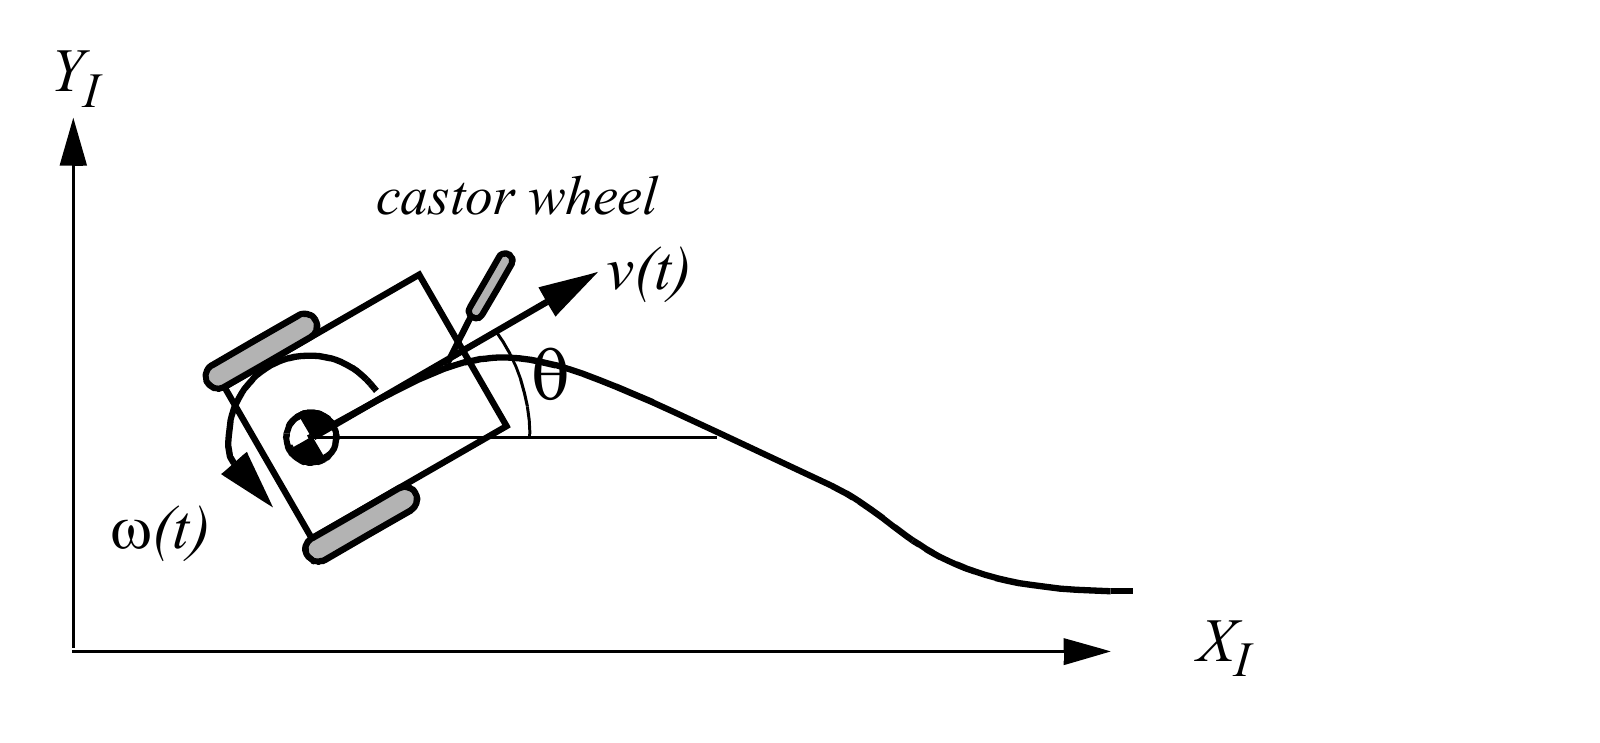
\includegraphics[width=\linewidth,height=4.5cm,keepaspectratio]{book_p078.png}\par}
\end{column}\begin{column}{0.49\textwidth}
Two fixed wheels, radius $r$, axle half-width $l$.\[J_1=\begin{bmatrix}1&0&l\\1&0&-l\end{bmatrix},\quad C_1=\begin{bmatrix}0&1&0\end{bmatrix}.\]\[\dot x_R=\frac r2(\dot\varphi_1+\dot\varphi_2),\quad\dot\theta=\frac r{2l}(\dot\varphi_1-\dot\varphi_2).\]Wheel labels follow the displayed rolling rows; positive spin drives forward. \begin{block}{Mobility}
$\dot y_R=0$; $\operatorname{rank}C_1=1$; $\delta_m=2$. Translation and rotation remain independent.
\end{block}\vspace{2mm}
\end{column}\end{columns}
\end{frame}

\begin{frame}[t]{Three Swedish wheels: no constraints at all}
\small
\setlength{\abovedisplayskip}{1mm}\setlength{\belowdisplayskip}{1mm}\setlength{\abovedisplayshortskip}{0pt}\setlength{\belowdisplayshortskip}{0pt}
\begin{columns}[T,onlytextwidth]\begin{column}{.49\textwidth}{\centering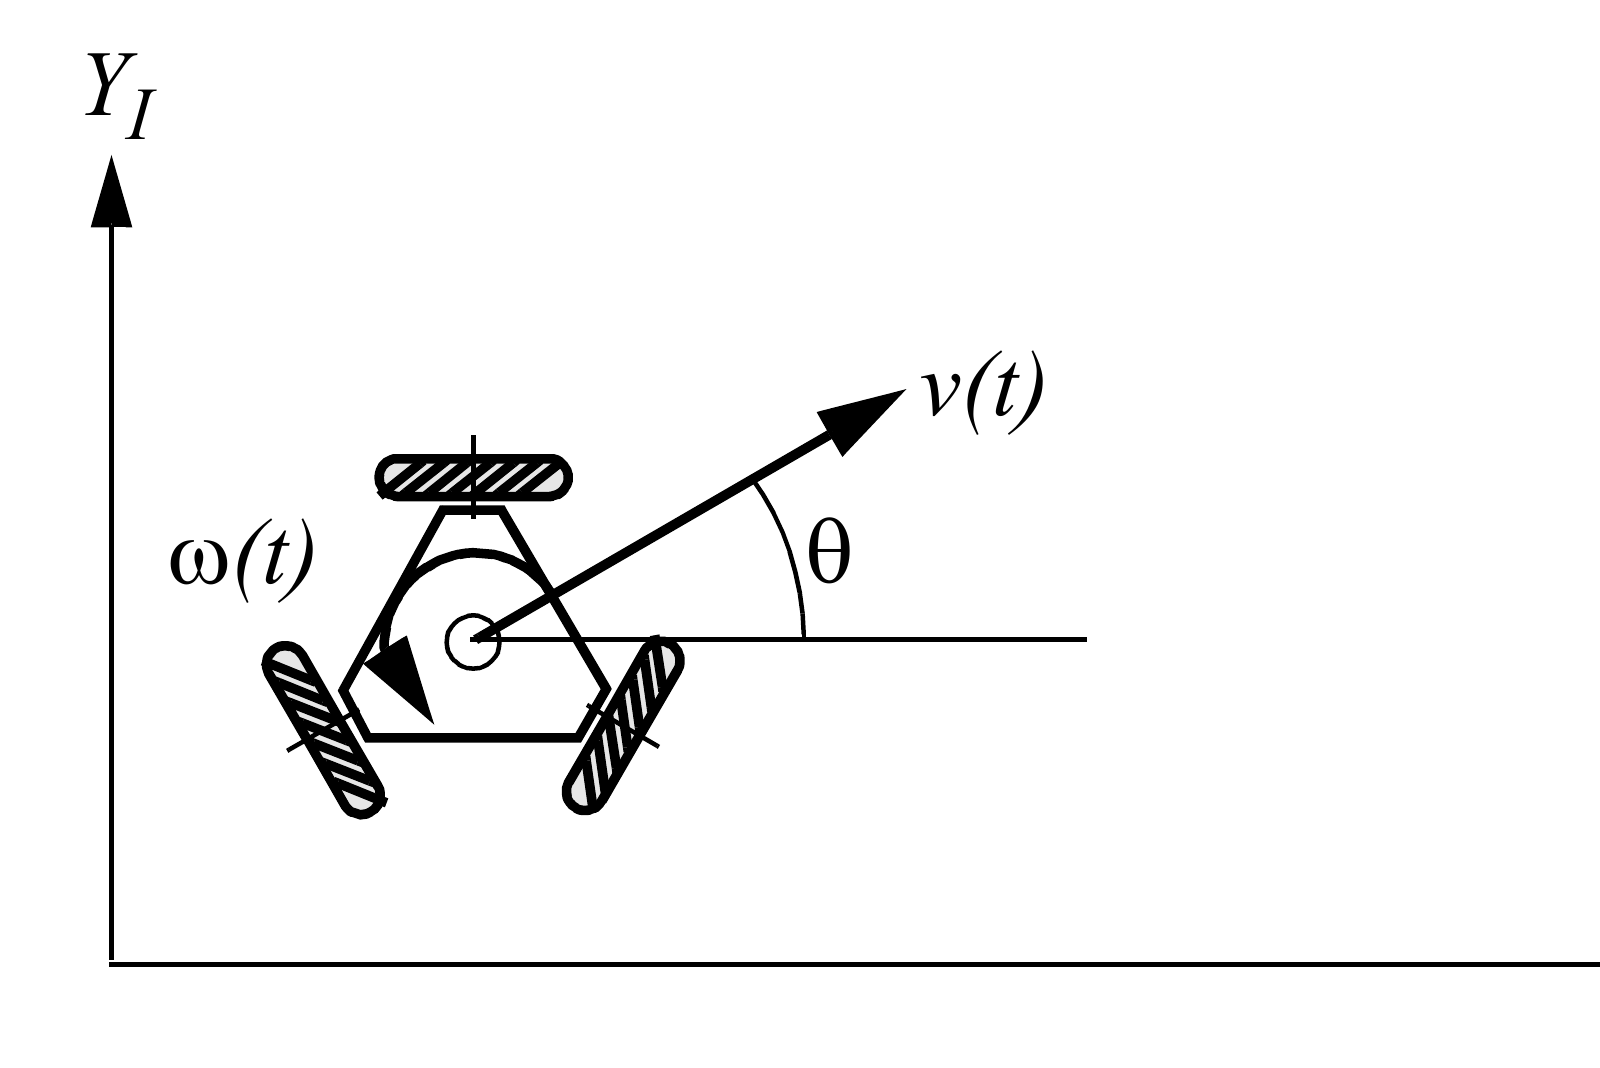
\includegraphics[width=\linewidth,height=3.6cm,keepaspectratio]{book_p091.png}\par}\end{column}\begin{column}{.49\textwidth}{\centering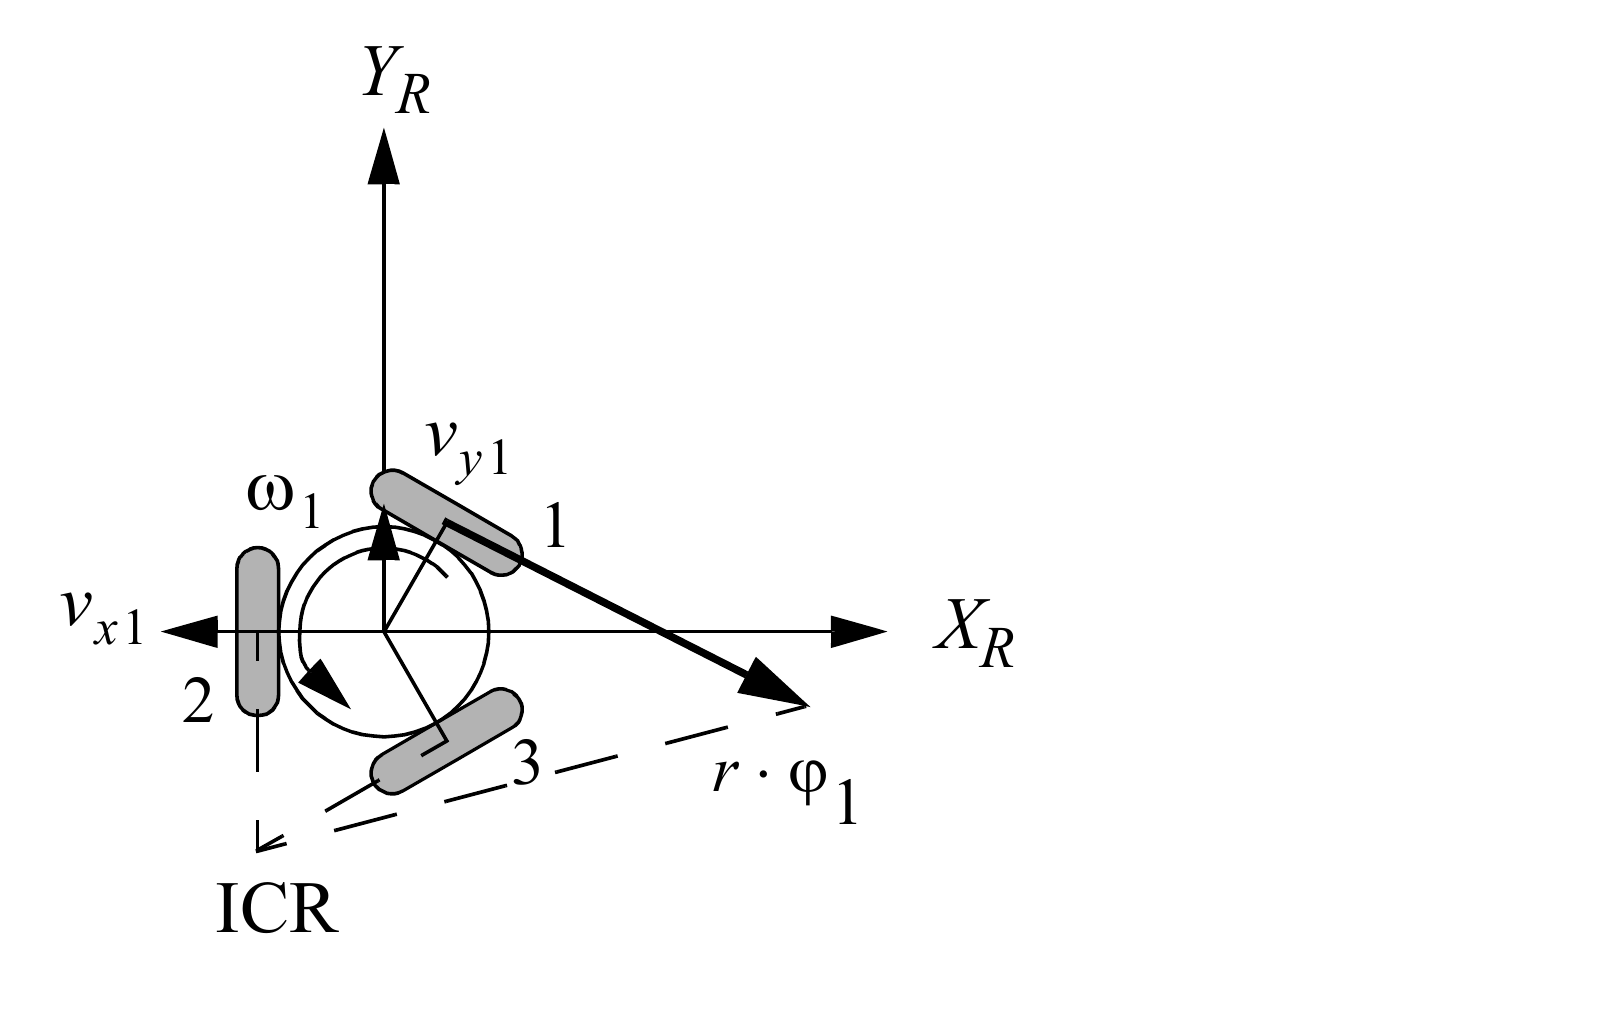
\includegraphics[width=\linewidth,height=3.6cm,keepaspectratio]{book_p092.png}\par}\end{column}\end{columns}\vspace{1.5mm}\par $\gamma=0$, $120^\circ$ spacing; $C_1$ empty, $\delta_m=3$. Any planar velocity: $\dot\xi_R=J_1^{-1}r\dot\varphi$.\[J_1=\begin{bmatrix}\sqrt3/2&-1/2&-l\\0&1&-l\\-\sqrt3/2&-1/2&-l\end{bmatrix},\qquad J_1^{-1}=\begin{bmatrix}1/\sqrt3&0&-1/\sqrt3\\-1/3&2/3&-1/3\\-1/(3l)&-1/(3l)&-1/(3l)\end{bmatrix}.\]
\end{frame}

\begin{frame}[t]{Differential drive plus a castor: nothing changes}
\small
\setlength{\abovedisplayskip}{1mm}\setlength{\belowdisplayskip}{1mm}
\setlength{\abovedisplayshortskip}{0pt}\setlength{\belowdisplayshortskip}{0pt}
\begin{columns}[T,onlytextwidth]\begin{column}{0.49\textwidth}
\centering\begin{tikzpicture}[scale=1.25]\draw[thick] (-1,-.7) rectangle (1,.7);\draw[fill=gray!40,thick](-.95,-.8) rectangle (-.25,-.6);\draw[fill=gray!40,thick](-.95,.6) rectangle (-.25,.8);\draw[dashed](-.6,-1.2)--(-.6,1.2);\draw[fill=gray!40](-.98,-.07) rectangle (-.76,.07);\draw[->](0,0)--(1.6,0) node[right]{$X_R$};\node at (0,-1.5){Two drive wheels + one free castor};\end{tikzpicture}\end{column}\begin{column}{0.49\textwidth}
\begin{block}{Support changes; mobility stays}
The castor adds wheel-spin and pivot variables, but no row to $C_1$. Thus $\operatorname{rank}C_1=1$ and $\delta_m=2$, just as before.
\end{block}\vspace{2mm}
\begin{block}{A fixed third wheel is different}
If its sliding row is independent, it further restricts the chassis. A suitably aligned redundant wheel adds no independent row.
\end{block}\vspace{2mm}
\end{column}\end{columns}
\end{frame}

\begin{frame}[t]{Mobility, steerability and manoeuvrability}
\small
\setlength{\abovedisplayskip}{1mm}\setlength{\belowdisplayskip}{1mm}\setlength{\abovedisplayshortskip}{0pt}\setlength{\belowdisplayshortskip}{0pt}
{\centering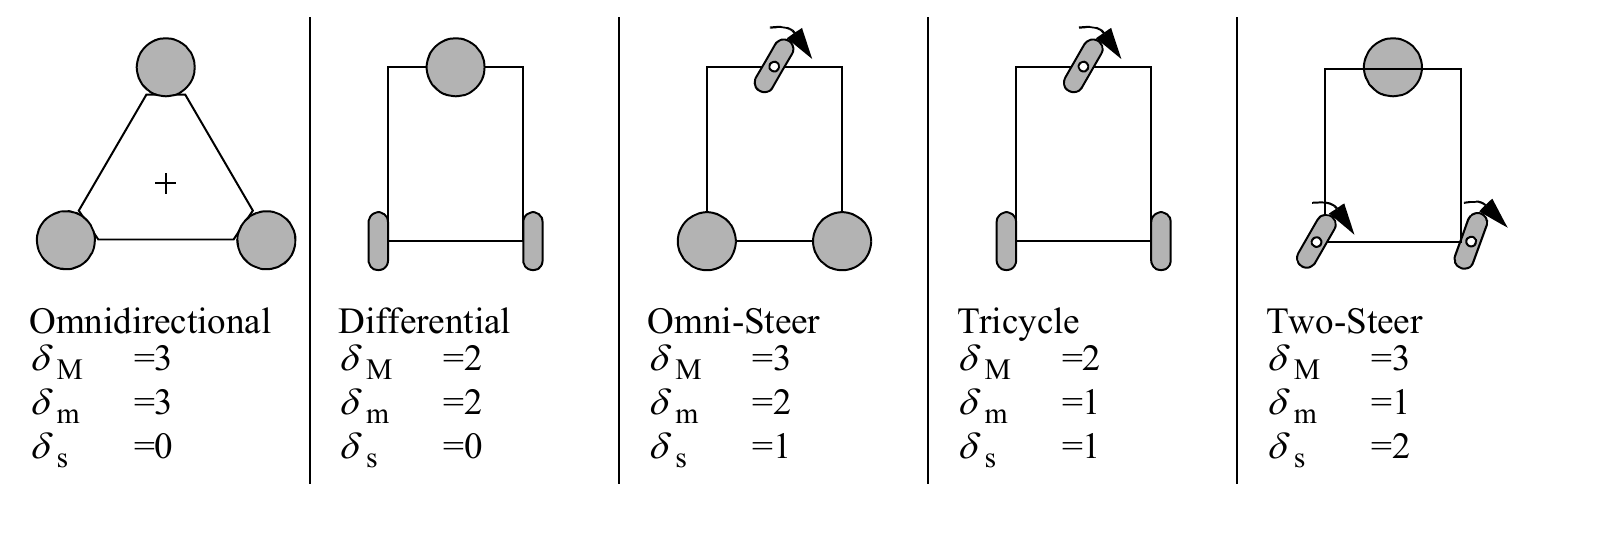
\includegraphics[width=\linewidth,height=3.3cm,keepaspectratio]{book_p100.png}\par}
\vspace{1.5mm}
\begin{columns}[T,onlytextwidth]\begin{column}{.55\textwidth}
\begin{tabularx}{\linewidth}{Xccccc}\toprule
Base & rank $C_1$ & $\delta_m$ & $\delta_s$ & $\delta_M$ & Sideways\\\midrule
Differential & 1 & 2 & 0 & 2 & no\\
Diff. + castor & 1 & 2 & 0 & 2 & no\\
Swedish & 0 & 3 & 0 & 3 & yes\\\bottomrule\end{tabularx}
\end{column}\begin{column}{.43\textwidth}
$\delta_m=3-\operatorname{rank}C_1$: independent velocities.\par
$\delta_s$: independent steering sets.\par
$\delta_M=\delta_m+\delta_s$: manoeuvrability.\par
Two-steer: $\delta_M=3$, not omni.
\end{column}\end{columns}
\end{frame}

\begin{frame}[t]{The reason is the instantaneous centre of rotation}
\small
\setlength{\abovedisplayskip}{1mm}\setlength{\belowdisplayskip}{1mm}\setlength{\abovedisplayshortskip}{0pt}\setlength{\belowdisplayshortskip}{0pt}
\begin{columns}[T,onlytextwidth]\begin{column}{.55\textwidth}{\centering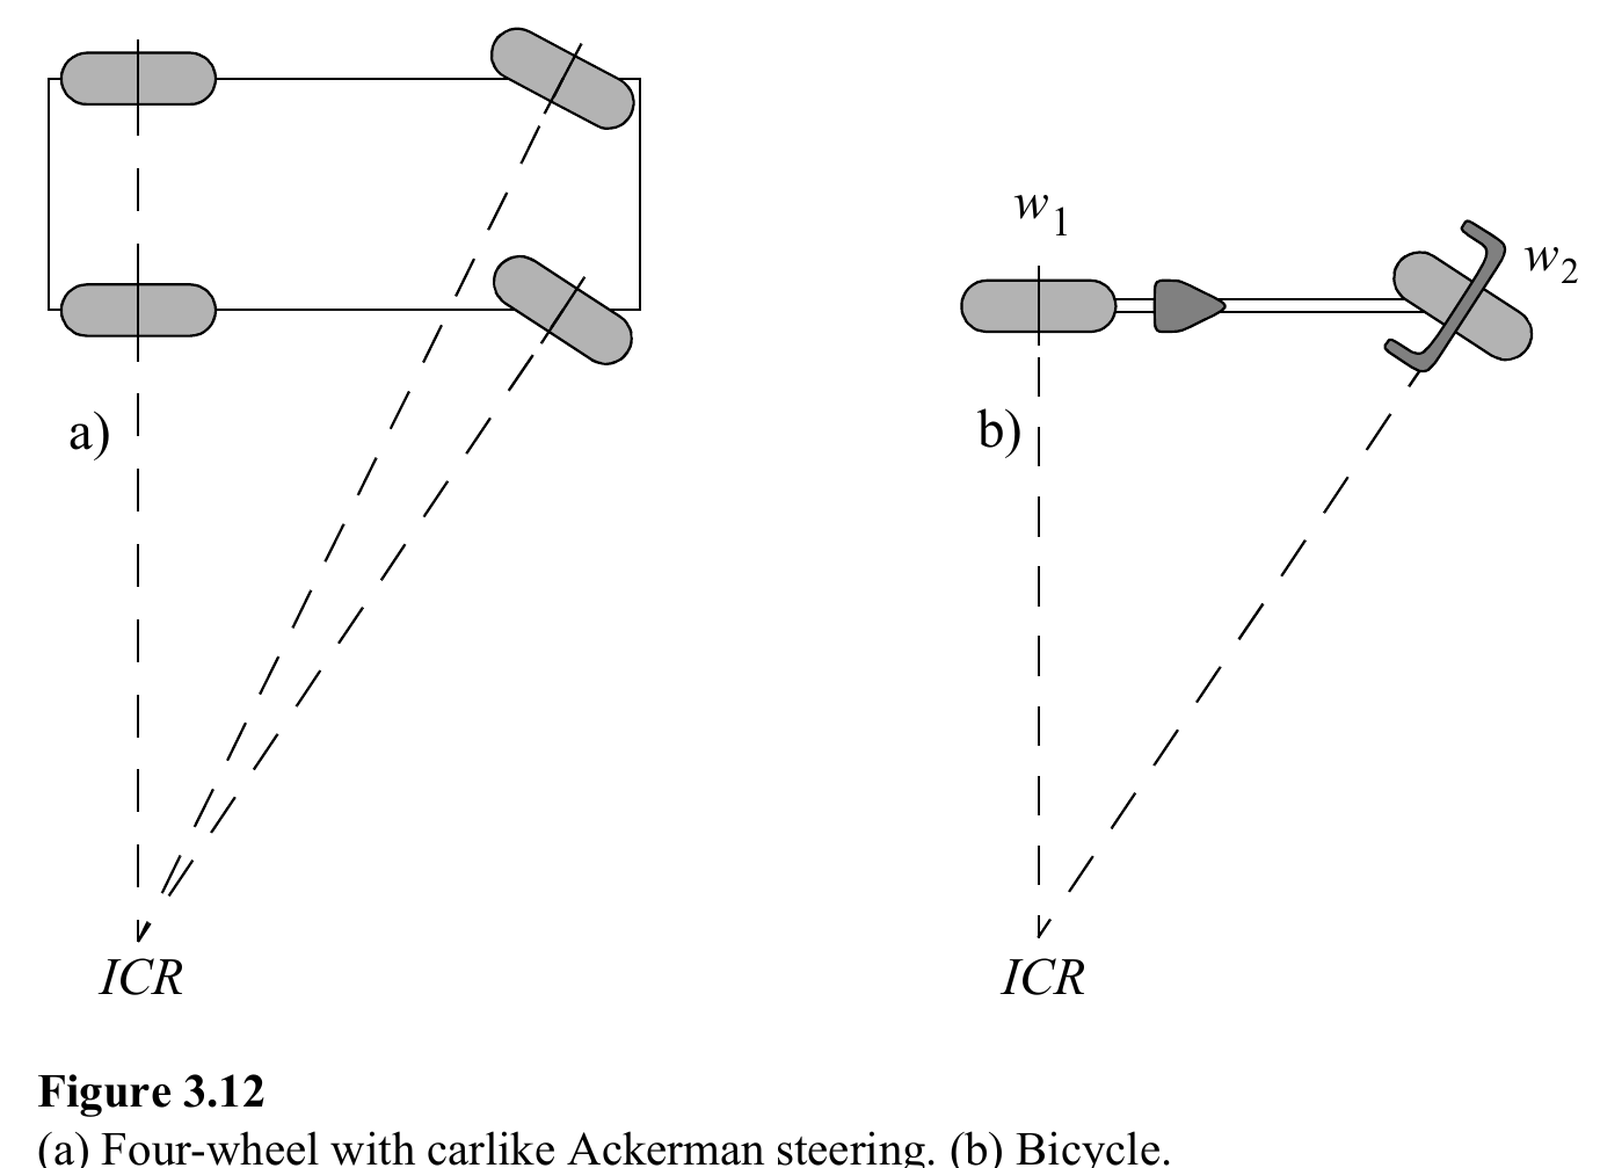
\includegraphics[width=\linewidth,height=5.5cm,keepaspectratio]{book_p095.png}\par}\end{column}\begin{column}{.43\textwidth}{\centering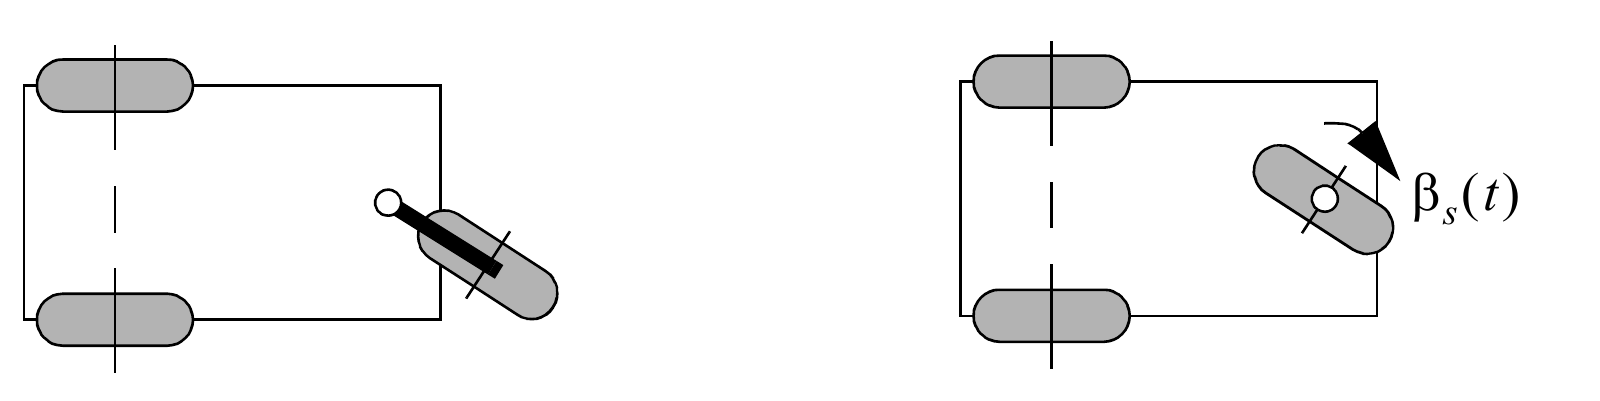
\includegraphics[width=\linewidth,height=2.2cm,keepaspectratio]{book_p096.png}\par}
{\centering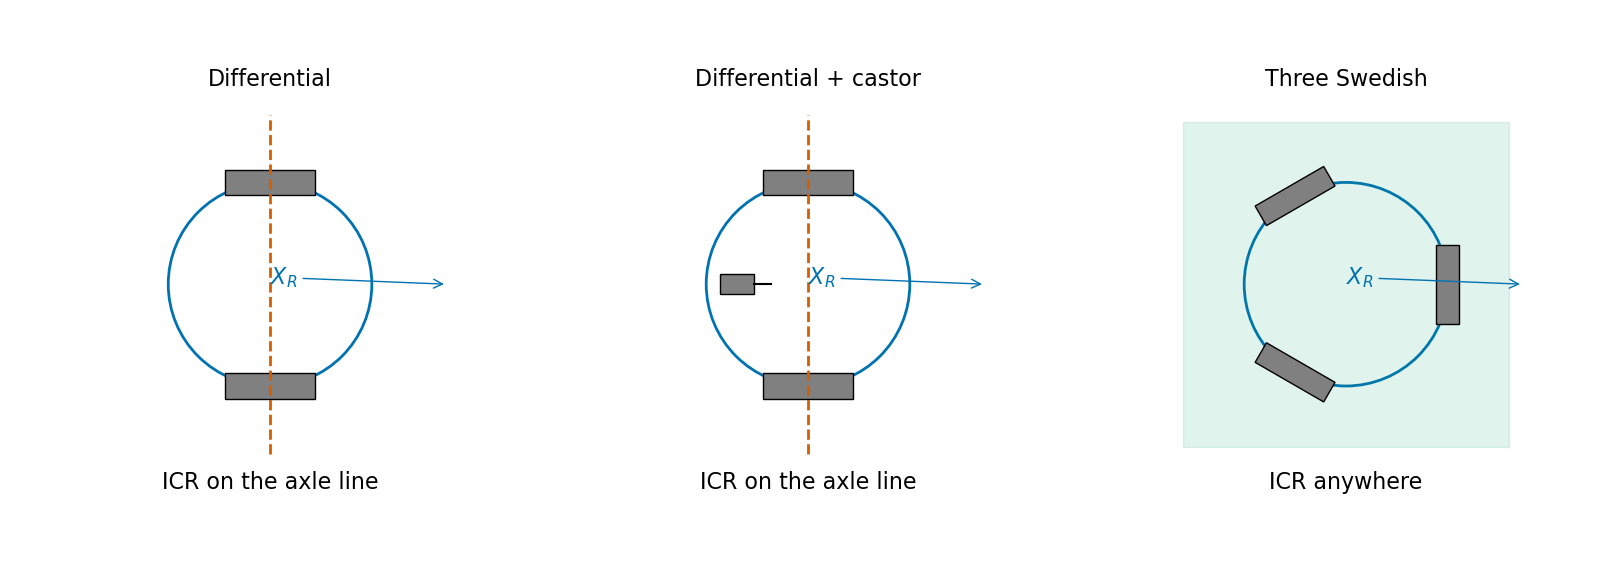
\includegraphics[width=\linewidth,height=3.0cm,keepaspectratio]{icr_three_bases.png}\par}

ICR: instantaneous centre of rotation. Fixed wheels require it on their axle line; omni permits it anywhere.\par
Straight travel: ICR at infinity. Rest: no unique ICR.
\end{column}\end{columns}
\end{frame}

\begin{frame}[t]{Control freedoms versus freedoms in the workspace}
\small
\setlength{\abovedisplayskip}{1mm}\setlength{\belowdisplayskip}{1mm}\setlength{\abovedisplayshortskip}{0pt}\setlength{\belowdisplayshortskip}{0pt}
{\centering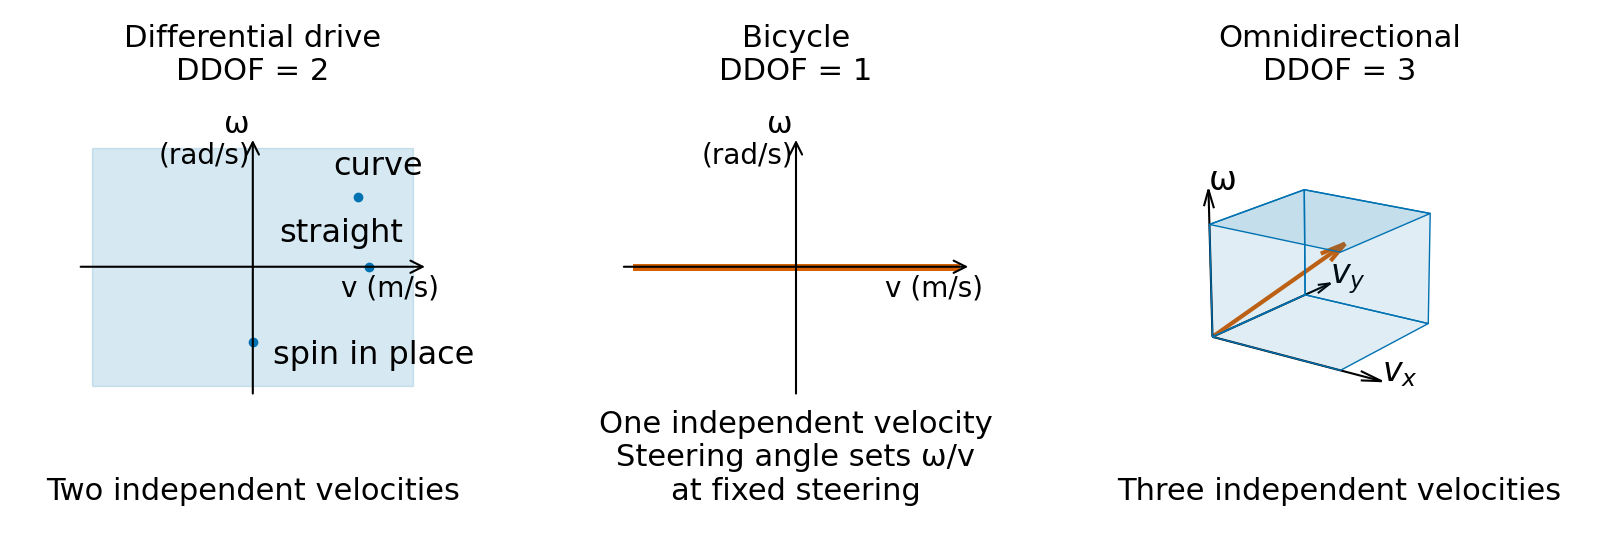
\includegraphics[width=\linewidth,height=3.9cm,keepaspectratio]{velocity_space.png}\par}\vspace{1.5mm}\par
\textbf{DDOF}: independent instantaneous velocities = $\delta_m$ (differential degrees of freedom).
\textbf{DOF}: dimension of reachable chassis poses. $\mathrm{DDOF}\leq\delta_M\leq\mathrm{DOF}$.\par
Bicycle: $(1,2,3)$; omni: $(3,3,3)$. Differential / unlocked Ackermann: DOF $=3$.\par
Configuration matters: synchro drive DOF $=2$; locked bicycle DOF $=1$.
\end{frame}

\begin{frame}[t]{Holonomic and nonholonomic constraints}
\small
\setlength{\abovedisplayskip}{1mm}\setlength{\belowdisplayskip}{1mm}
\setlength{\abovedisplayshortskip}{0pt}\setlength{\belowdisplayshortskip}{0pt}
\begin{block}{Holonomic: a position rule}
A constraint is \textbf{holonomic} if it can be written using positions only. \textbf{Integrable} means a velocity rule is secretly a rule about position.
\end{block}\vspace{2mm}
\begin{block}{Nonholonomic: a velocity rule that cannot be integrated}
A fixed wheel forbids sideways velocity, not sideways displacement reached by manoeuvring.\[-\sin\theta\,\dot x+\cos\theta\,\dot y=0.\]
\end{block}\vspace{2mm}
Turning, driving, then turning can reach a sideways pose. The sliding rule is therefore nonholonomic; it cannot be replaced by one position-only condition for the mobile base.
\end{frame}

\begin{frame}[t]{Locked bicycle, and the DDOF = DOF test}
\small
\setlength{\abovedisplayskip}{1mm}\setlength{\belowdisplayskip}{1mm}
\setlength{\abovedisplayshortskip}{0pt}\setlength{\belowdisplayshortskip}{0pt}
\textbf{DDOF}: differential degrees of freedom = independent instantaneous velocities the robot can set = $\delta_m$. \textbf{DOF}: dimension of reachable poses.\par\vspace{2mm}\begin{columns}[T,onlytextwidth]\begin{column}{0.49\textwidth}
\begin{block}{Lock the bicycle steering straight}
Two parallel fixed wheels lie one behind the other. With the initial line chosen as $X$, the constraints become $y=0$, $\theta=0$; rolling gives $\varphi=x/r+\varphi_0$. Here $\varphi_0$ is initial wheel rotation.
\end{block}\vspace{2mm}
All restrictions are integrable. Only translation along the line remains.\end{column}\begin{column}{0.49\textwidth}
\begin{block}{A clean chassis-level test}
\[\text{holonomic}\quad\Longleftrightarrow\quad\mathrm{DDOF}=\mathrm{DOF}.\] Locked bicycle: $1=1$, holonomic but not omni.
\end{block}\vspace{2mm}
\begin{block}{Omnidirectional}
Holonomic with DDOF $=3$: arbitrary planar translation and rotation are immediately available.
\end{block}\vspace{2mm}
\end{column}\end{columns}
\end{frame}

\begin{frame}[t]{Our bases on the holonomic scale}
\small
\setlength{\abovedisplayskip}{1mm}\setlength{\belowdisplayskip}{1mm}
\setlength{\abovedisplayshortskip}{0pt}\setlength{\belowdisplayshortskip}{0pt}
\begin{columns}[T,onlytextwidth]\begin{column}{0.49\textwidth}
\renewcommand{\arraystretch}{1.1}\begin{tabularx}{\linewidth}{Xcccc}
\toprule Base & DDOF & DOF & Holo. & Omni\\\midrule
Differential & 2 & 3 & no & no\\
Diff. + castor & 2 & 3 & no & no\\
Swedish omni & 3 & 3 & yes & yes\\
Ackermann & 1 & 3 & no & no\\\bottomrule\end{tabularx}
\vspace{3mm}\par More instantaneous freedoms mean fewer preparatory manoeuvres.\end{column}\begin{column}{0.49\textwidth}
{\centering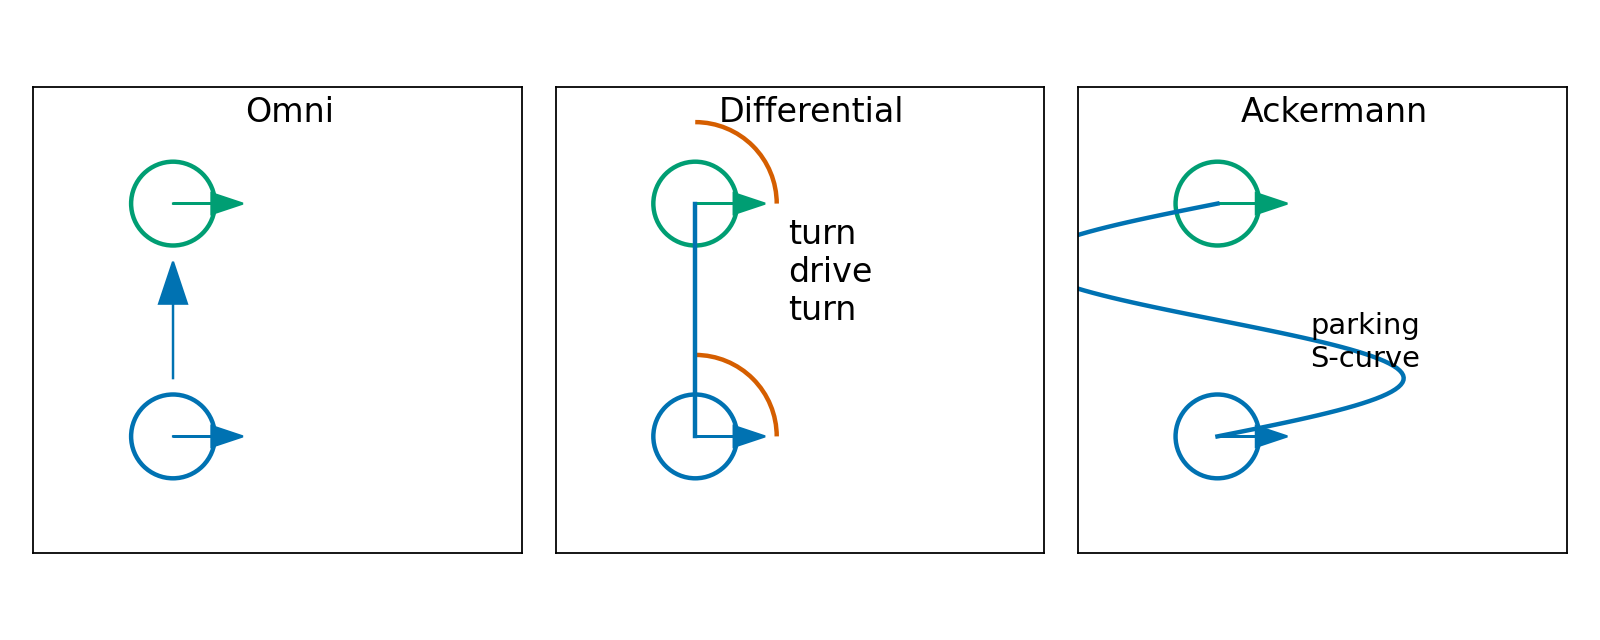
\includegraphics[width=\linewidth,height=4.5cm,keepaspectratio]{lateral_move.png}\par}
Same sideways displacement, different motion sequences.\end{column}\end{columns}
\end{frame}

\begin{frame}[t]{Path versus trajectory}
\small
\setlength{\abovedisplayskip}{1mm}\setlength{\belowdisplayskip}{1mm}
\setlength{\abovedisplayshortskip}{0pt}\setlength{\belowdisplayshortskip}{0pt}
\begin{columns}[T,onlytextwidth]\begin{column}{0.49\textwidth}
{\centering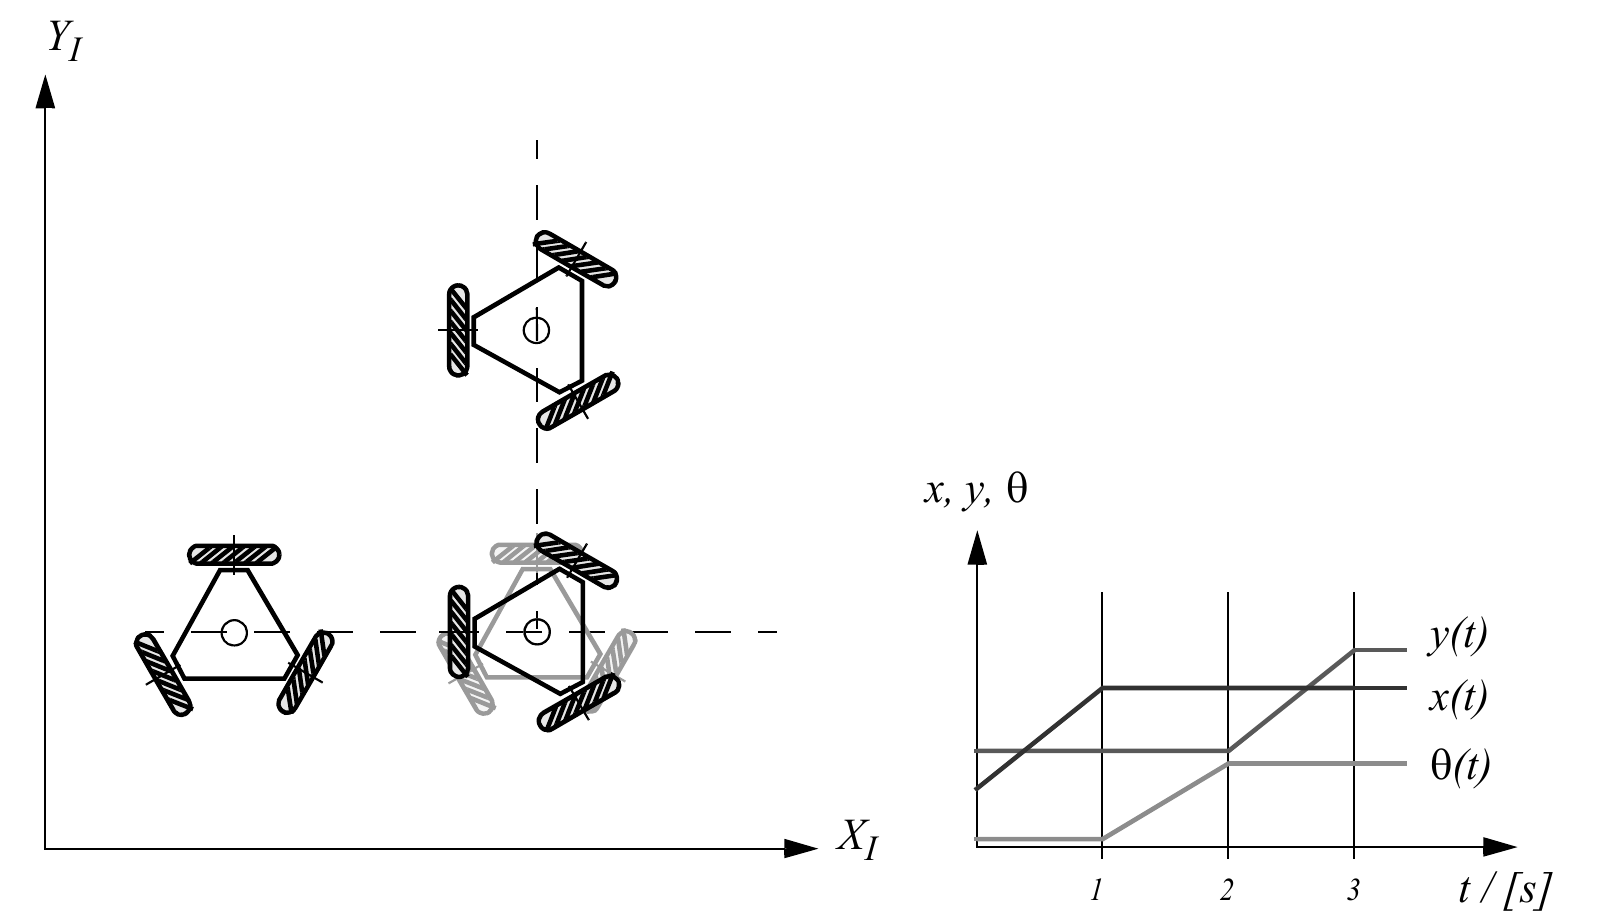
\includegraphics[width=\linewidth,height=4.5cm,keepaspectratio]{book_p105.png}\par}
\end{column}\begin{column}{0.49\textwidth}
\begin{block}{Path and trajectory}
A \textbf{path} is a trace in pose space $(x,y,\theta)$. A \textbf{trajectory} adds time: $(x,y,\theta,t)$.
\end{block}\vspace{2mm}
Three phases: 1 s along $X$ at 1 m/s; 1 s rotating by $90^\circ$; 1 s along $Y$ at 1 m/s.\vspace{2mm}\par An omni can follow this ideal trajectory exactly by changing wheel speeds at the switches. Infinite acceleration is assumed.\end{column}\end{columns}
\end{frame}

\begin{frame}[t]{Two-steer cannot follow the same trajectory}
\small
\setlength{\abovedisplayskip}{1mm}\setlength{\belowdisplayskip}{1mm}\setlength{\abovedisplayshortskip}{0pt}\setlength{\belowdisplayshortskip}{0pt}
\begin{columns}[T,onlytextwidth]\begin{column}{.49\textwidth}{\centering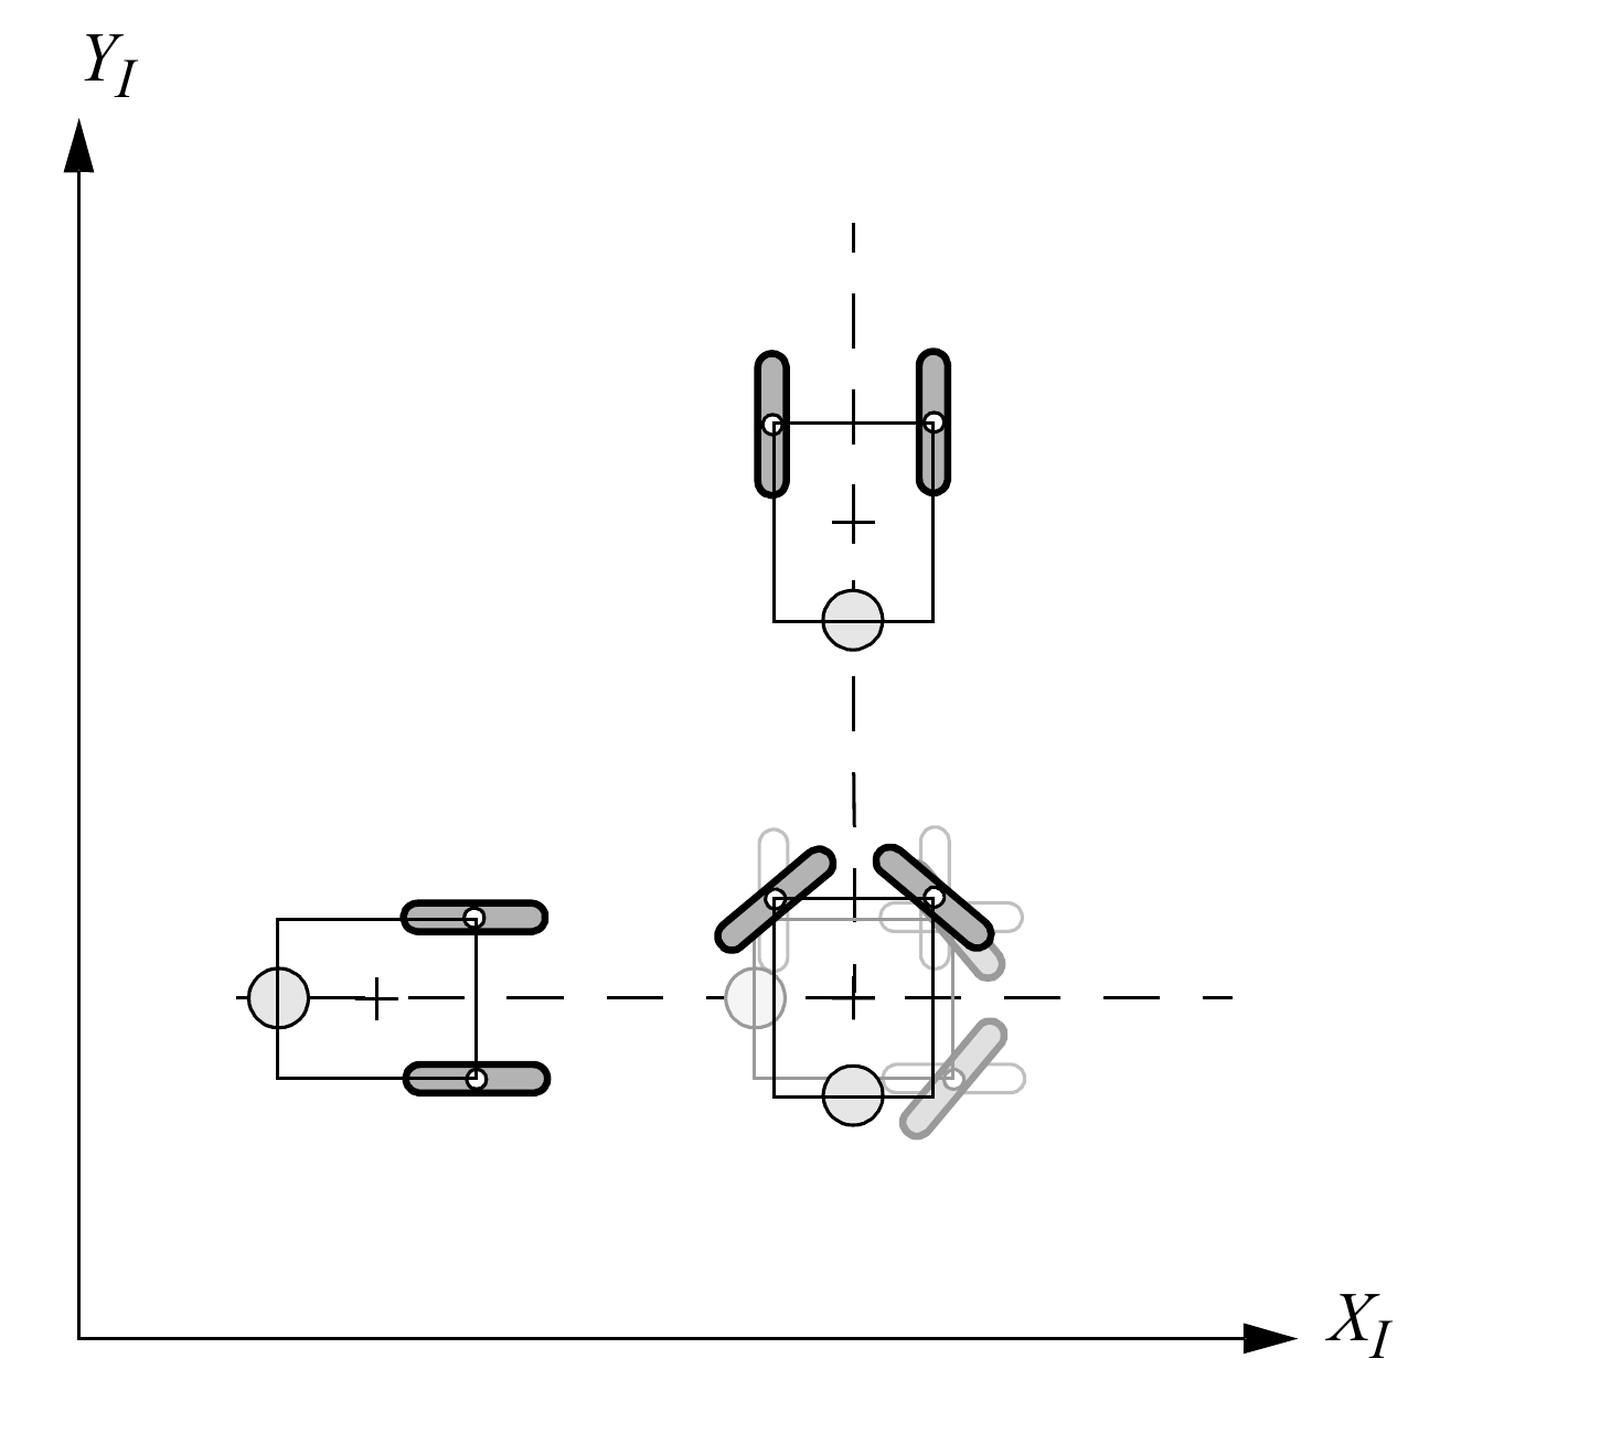
\includegraphics[width=\linewidth,height=5.5cm,keepaspectratio]{book_p106_motion.png}\par}\end{column}\begin{column}{.49\textwidth}{\centering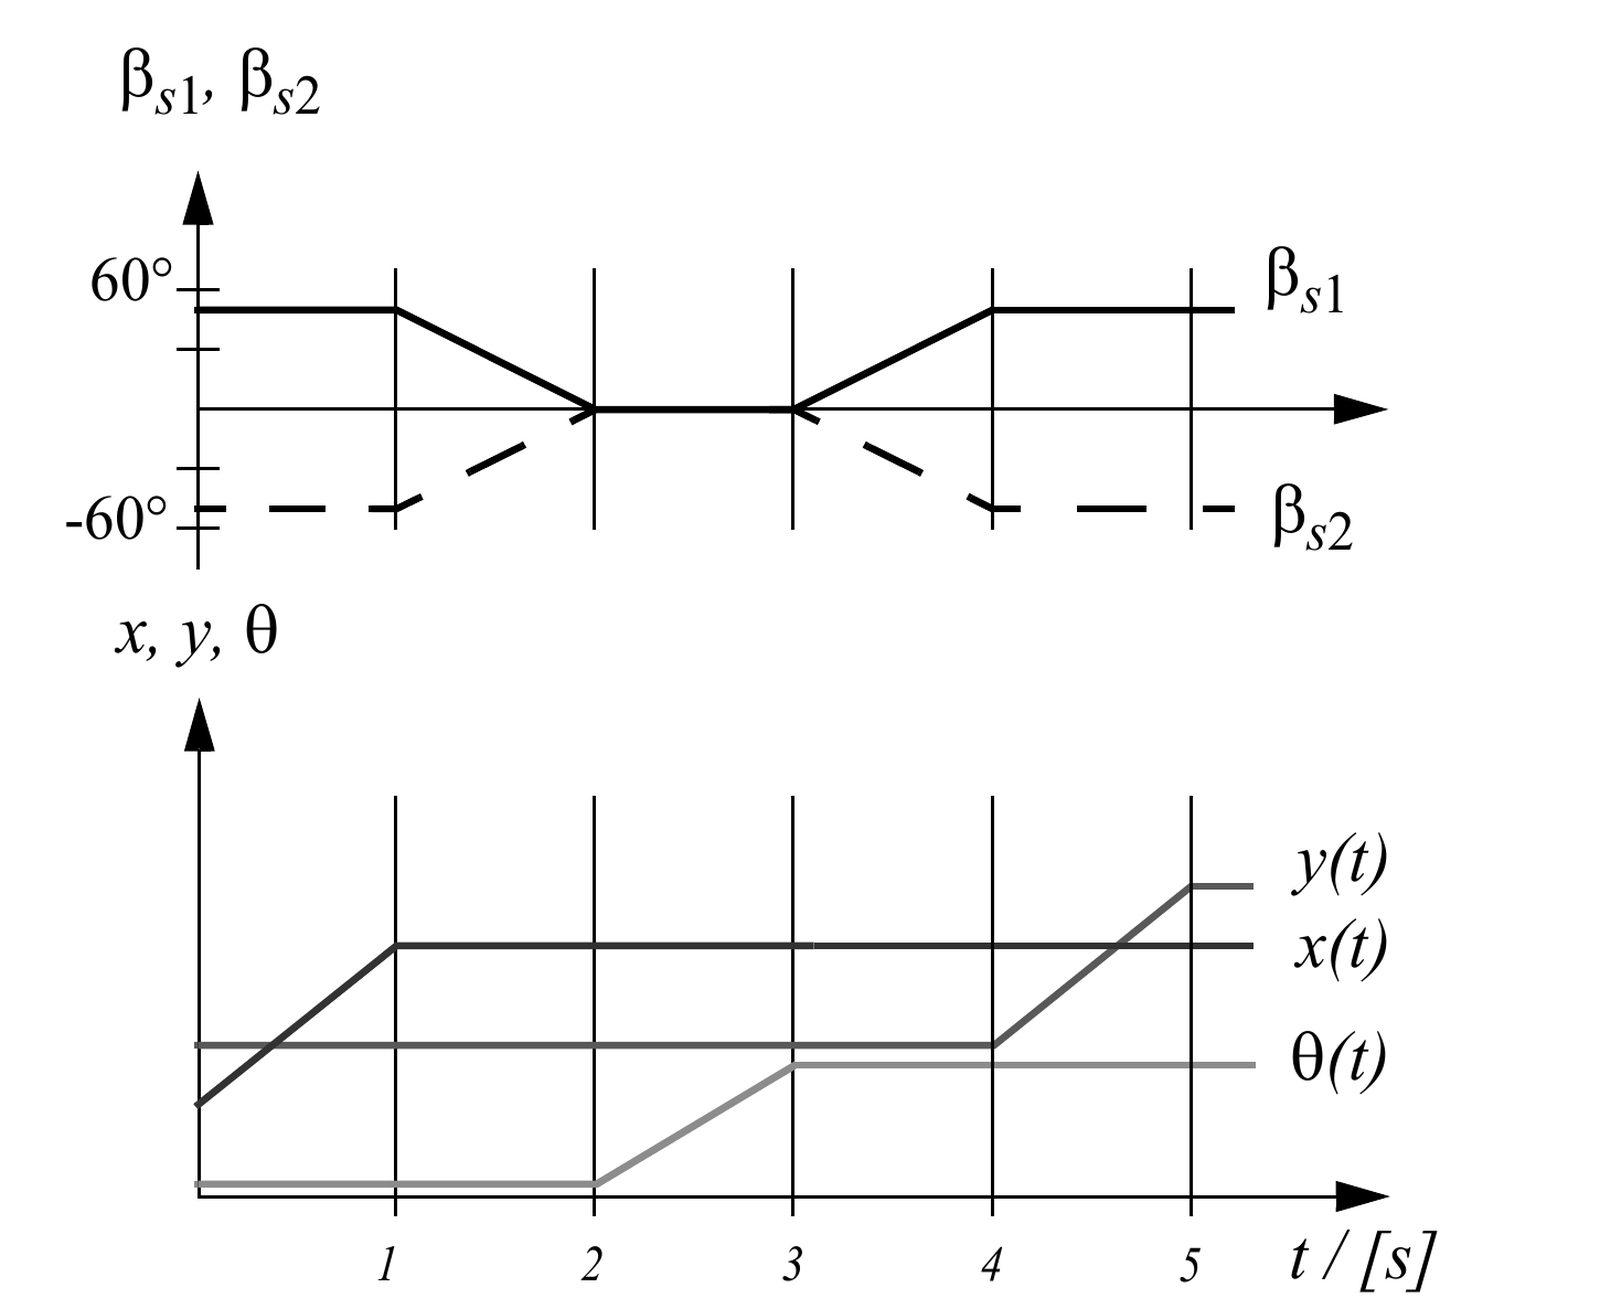
\includegraphics[width=\linewidth,height=5.5cm,keepaspectratio]{book_p106_timing.png}\par}\end{column}\end{columns}\vspace{1.5mm}\par $\delta_M=3$: same path, but steering takes time. Three motion phases + two steering phases = five.
\end{frame}

\begin{frame}[t]{Why not omni everywhere, and what kinematics leaves out}
\small
\setlength{\abovedisplayskip}{1mm}\setlength{\belowdisplayskip}{1mm}
\setlength{\abovedisplayshortskip}{0pt}\setlength{\belowdisplayshortskip}{0pt}
\begin{columns}[T,onlytextwidth]\begin{column}{0.49\textwidth}
\begin{block}{Omni has physical costs}
Roller wheels are complex and expensive. Ground clearance and suspension are harder to provide.
\end{block}\vspace{2mm}
In a fast curve, car-like sliding constraints carry lateral force passively. An omni must supply lateral force through motor torque; it may be thrown out of the curve.\end{column}\begin{column}{0.49\textwidth}
\begin{block}{Kinematics describes possible velocities}
Dynamics adds mass, inertia and force. \textbf{Motorization} concerns the forces and torques the motors must supply. Controllability asks whether the available commands can produce the required motion.
\end{block}\vspace{2mm}
A feasible geometric path still needs a controller that can execute it.\end{column}\end{columns}
\end{frame}

\begin{frame}[t]{Open loop: lines and arcs, and why it is not enough}
\small
\setlength{\abovedisplayskip}{1mm}\setlength{\belowdisplayskip}{1mm}
\setlength{\abovedisplayshortskip}{0pt}\setlength{\belowdisplayshortskip}{0pt}
\begin{columns}[T,onlytextwidth]\begin{column}{0.49\textwidth}\centering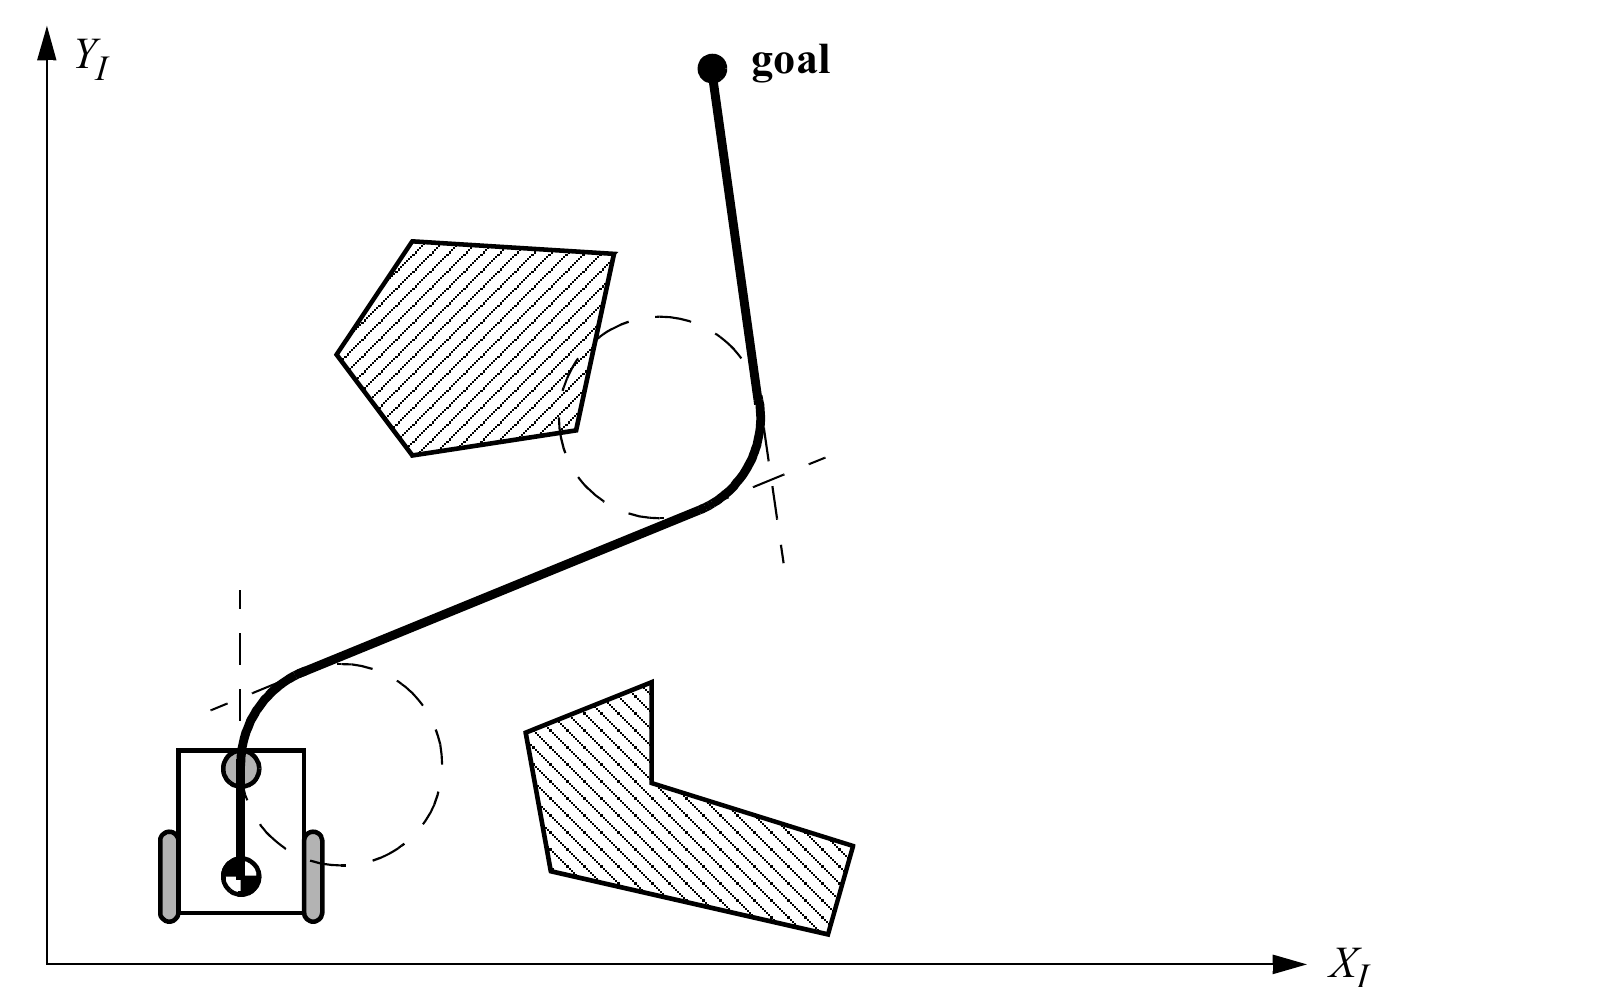
\includegraphics[width=\linewidth,height=4.5cm,keepaspectratio]{book_p108.png}\par\end{column}\begin{column}{0.49\textwidth}\textbf{Open loop}: precompute straight segments and arcs; do not feed measured pose back. A segment is one piece of the route.\par\vspace{3mm}Three weaknesses:\begin{enumerate}\item Feasibility is hard to precompute with speed and acceleration limits.\item No adaptation to environment changes.\item Nonsmooth transitions cause acceleration jumps.\end{enumerate}\end{column}\end{columns}
\end{frame}

\begin{frame}[t]{Feedback control: the pose error and why a gain matrix fails}
\small
\setlength{\abovedisplayskip}{1mm}\setlength{\belowdisplayskip}{1mm}
\setlength{\abovedisplayshortskip}{0pt}\setlength{\belowdisplayshortskip}{0pt}
\begin{columns}[T,onlytextwidth]\begin{column}{0.49\textwidth}
{\centering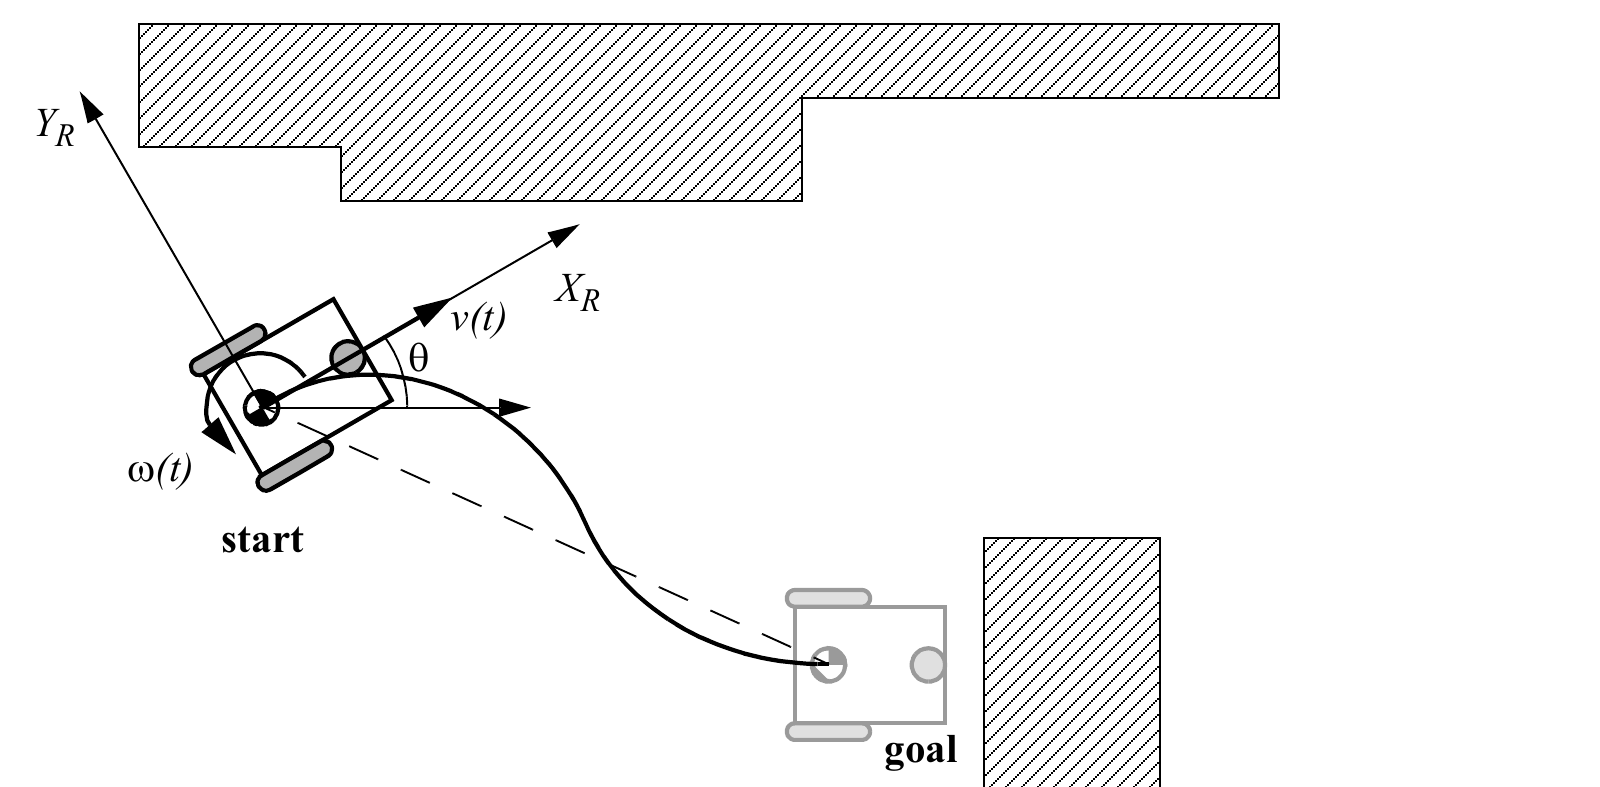
\includegraphics[width=\linewidth,height=2.8cm,keepaspectratio]{book_p109.png}\par}
$e=(\Delta x,\Delta y,\Delta\theta)^T$: pose error in the robot coordinate frame. A $2\times3$ gain matrix $K$ suggests $(v,\omega)^T=Ke$.\end{column}\begin{column}{0.49\textwidth}
$v$: forward speed; $\omega$: yaw rate.\[\dot x=v\cos\theta,\quad\dot y=v\sin\theta,\quad\dot\theta=\omega.\]Two inputs control three pose outputs. Sideways error first needs a change in heading.\begin{block}{The smooth-feedback obstruction}
No smooth time-invariant state feedback defined around the goal asymptotically stabilises the full pose. Polar feedback avoids this restriction because its Cartesian form is undefined at $\rho=0$.
\end{block}\vspace{2mm}
\end{column}\end{columns}
\end{frame}

\begin{frame}[t]{Polar coordinates around the goal}
\small
\setlength{\abovedisplayskip}{1mm}\setlength{\belowdisplayskip}{1mm}\setlength{\abovedisplayshortskip}{0pt}\setlength{\belowdisplayshortskip}{0pt}
\begin{columns}[T,onlytextwidth]\begin{column}{.65\textwidth}
{\centering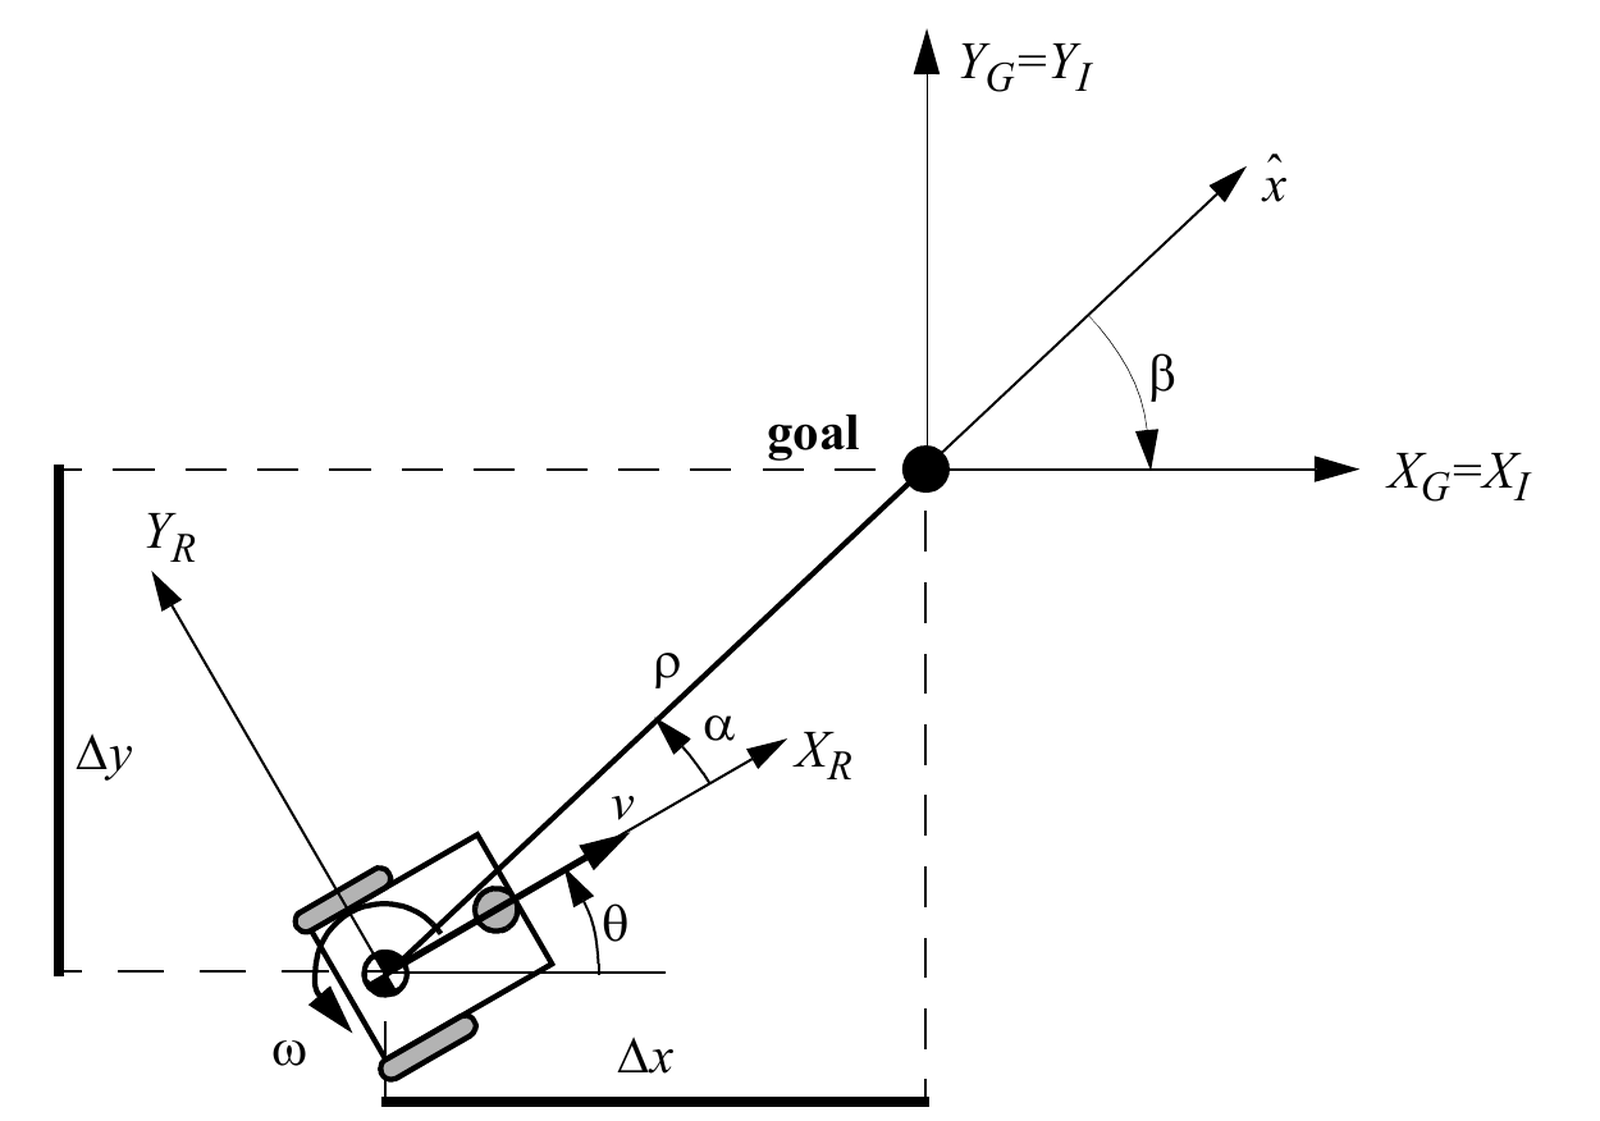
\includegraphics[width=\linewidth,height=6cm,keepaspectratio]{book_p110.png}\par}
\end{column}\begin{column}{.33\textwidth}
Goal at origin, heading $0$; robot heading $\theta$.\par
Global displacements:\par $\Delta x=x_g-x$, $\Delta y=y_g-y$.\par
$\rho=\sqrt{\Delta x^2+\Delta y^2}$:\par distance to goal.\par
$\lambda=\operatorname{atan2}(\Delta y,\Delta x)$:\par goal bearing.\par
$\alpha=\operatorname{wrap}(\lambda-\theta)$:\par heading to goal line.\par
$\beta=\operatorname{wrap}(-\theta-\alpha)$:\par goal line to goal heading.\par
Wrap angles to $(-\pi,\pi]$.
\end{column}\end{columns}
\end{frame}

\begin{frame}[t]{The model in polar coordinates, and its limits}
\small
\setlength{\abovedisplayskip}{1mm}\setlength{\belowdisplayskip}{1mm}
\setlength{\abovedisplayshortskip}{0pt}\setlength{\belowdisplayshortskip}{0pt}
\begin{columns}[T,onlytextwidth]\begin{column}{0.49\textwidth}\textbf{Forward: goal in front}\[\begin{aligned}\dot\rho&=-v\cos\alpha,\\\dot\alpha&=v\sin\alpha/\rho-\omega,\\\dot\beta&=-v\sin\alpha/\rho.\end{aligned}\]$I_1=(-\pi/2,\pi/2]$ is the forward sector. Choose direction at $t=0$, once.\par\vspace{2mm}\textbf{Reverse: physical $v=-v_c$, $v_c\geq0$}\[\begin{aligned}\dot\rho&=v_c\cos\alpha,\\\dot\alpha&=-v_c\sin\alpha/\rho-\omega,\\\dot\beta&=v_c\sin\alpha/\rho.\end{aligned}\]\end{column}\begin{column}{0.49\textwidth}For a goal behind, flip both headings:\[\theta\prime=\theta+\pi,\qquad\phi\prime=\phi+\pi.\]$\phi$ is requested goal heading; positions stay fixed.\[\begin{aligned}\alpha\prime&=\operatorname{wrap}(\alpha-\pi),\\\beta\prime&=\operatorname{wrap}(\beta+\pi).\end{aligned}\]Use the forward law on primed errors; physical commands are $(-v_c,\omega_c)$. Same relative heading: requested pose, rear-first.\par\vspace{2mm}At $\rho=0$ the transform is undefined. Stop on position \emph{and} heading tolerance.\end{column}\end{columns}
\end{frame}

\begin{frame}[t]{The control law and the closed loop}
\small
\setlength{\abovedisplayskip}{1mm}\setlength{\belowdisplayskip}{1mm}
\setlength{\abovedisplayshortskip}{0pt}\setlength{\belowdisplayshortskip}{0pt}
\begin{columns}[T,onlytextwidth]\begin{column}{0.49\textwidth}\textbf{Forward-mode feedback}\[v=k_\rho\rho,\qquad\omega=k_\alpha\alpha+k_\beta\beta.\]A gain $k$ sets reaction strength.\par\vspace{2mm}Distance sets speed; $\alpha$ turns toward the goal; $\beta$ aligns final heading.\par\vspace{2mm}Reverse: same law on primed errors, physical $v=-k_\rho\rho$.\end{column}\begin{column}{0.49\textwidth}\textbf{Closed loop}\[\begin{aligned}\dot\rho&=-k_\rho\rho\cos\alpha,\\\dot\alpha&=k_\rho\sin\alpha-k_\alpha\alpha-k_\beta\beta,\\\dot\beta&=-k_\rho\sin\alpha.\end{aligned}\]No singular term remains in these equations. With stabilising gains, the goal equilibrium is $(\rho,\alpha,\beta)=(0,0,0)$.\end{column}\end{columns}
\end{frame}

\begin{frame}[t]{Stability conditions and how to read the gains}
\small
\setlength{\abovedisplayskip}{1mm}\setlength{\belowdisplayskip}{1mm}\setlength{\abovedisplayshortskip}{0pt}\setlength{\belowdisplayshortskip}{0pt}
\textbf{Local exponential stability}
\[k_\rho>0,\qquad k_\beta<0,\qquad k_\alpha>k_\rho.\]
\vspace{1.5mm}\par\textbf{Sufficient sector condition: retain the chosen direction}
\[k_\alpha>\frac{2k_\rho}{\pi}+2|k_\beta|.\]
With local conditions: inward $\dot\alpha$ at $\alpha=\pm\pi/2$ for every wrapped $\beta$; primed in reverse.
\[\left.\dot\alpha\right|_{\alpha=\pi/2}\leq k_\rho+|k_\beta|\pi-k_\alpha\pi/2<0.\]
\textbf{Intuition:} $k_\rho$ sets speed; too large exceeds wheel limits. $k_\alpha>k_\rho$ turns faster than approach. $k_\beta<0$ aligns final heading.\par\vspace{1.5mm}
Book gains $(3,8,-1.5)$: $2k_\rho/\pi+2|k_\beta|\approx4.91<8$.
\end{frame}

\begin{frame}[t]{Demo 1: choose the gains yourself}
\small
\vspace{-1mm}
{\centering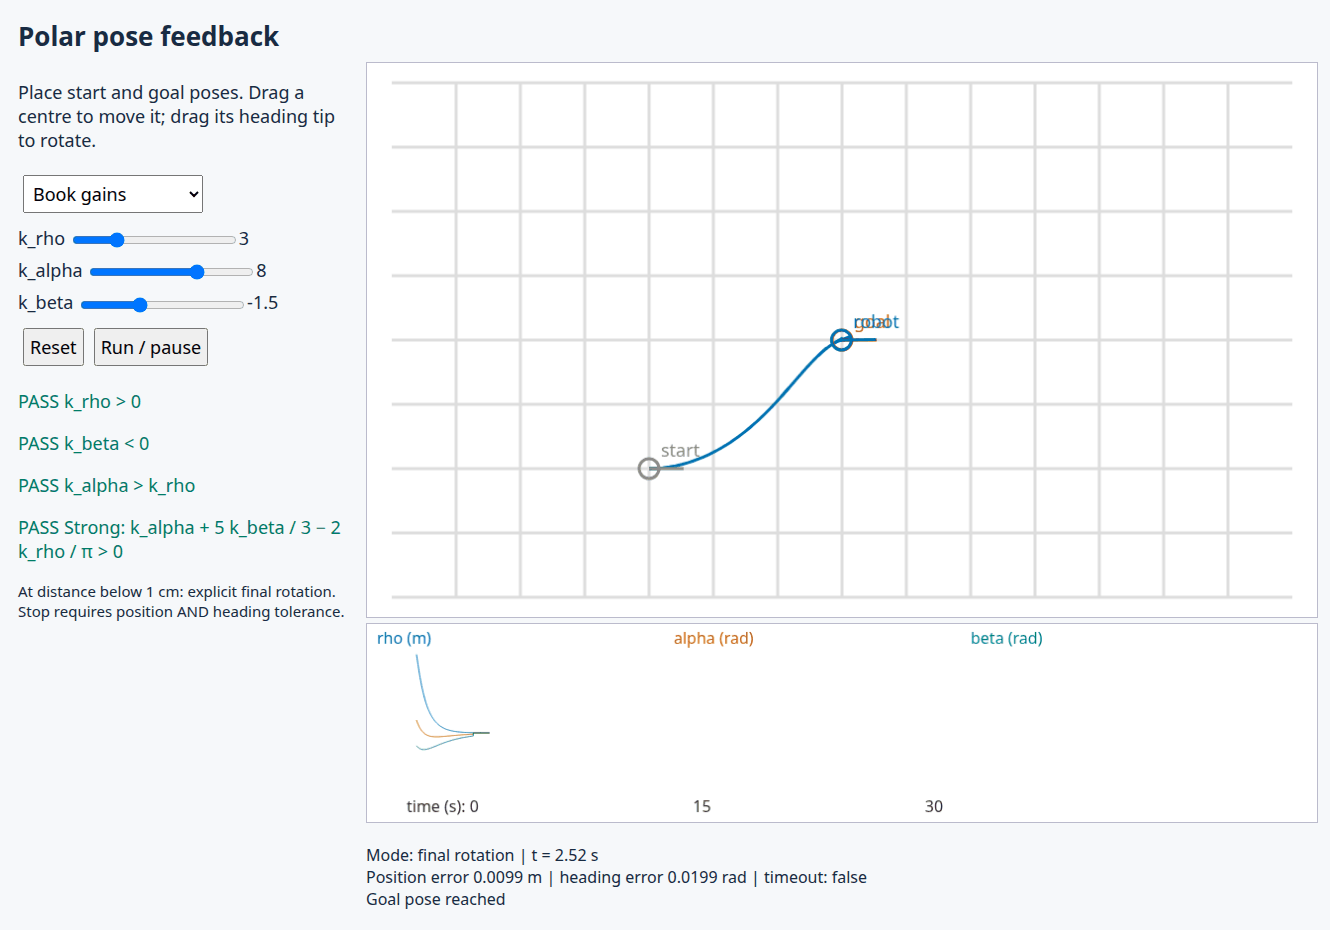
\includegraphics[width=\linewidth,height=5.5cm,keepaspectratio]{polar_demo_capture.png}\par}Book gains $(3,8,-1.5)$; vary gains and watch position, final heading and stability. \texttt{pixi run serve}.
\end{frame}

\begin{frame}[t]{What this controller does not know:\\pose stabiliser versus path tracker}
\small
\setlength{\abovedisplayskip}{1mm}\setlength{\belowdisplayskip}{1mm}
\setlength{\abovedisplayshortskip}{0pt}\setlength{\belowdisplayshortskip}{0pt}
\begin{columns}[T,onlytextwidth]\begin{column}{0.49\textwidth}
\begin{block}{Pose stabiliser}
One requested goal pose. Differential-drive kinematics. No obstacles or acceleration limits in the model.
\end{block}\vspace{2mm}
It reaches a pose without deciding which side of a wall to use.\end{column}\begin{column}{0.49\textwidth}
\begin{block}{The two missing roles}
A \textbf{global planner} finds the route around walls. A \textbf{local planner} tracks it while reacting to nearby obstacles.
\end{block}\vspace{2mm}
Nav2 local controllers are path trackers with obstacle awareness. Feedback idea: measure error, command $(v,\omega)$, repeat. The polar formulas are not used. Default: 20 Hz.\par\vspace{1mm}{\scriptsize Defaults in the Nav2 repository; check your release.}\end{column}\end{columns}
\end{frame}

\begin{frame}[t]{Navigation as two loops:\\planner server and controller server}
\small
\setlength{\abovedisplayskip}{1mm}\setlength{\belowdisplayskip}{1mm}
{\centering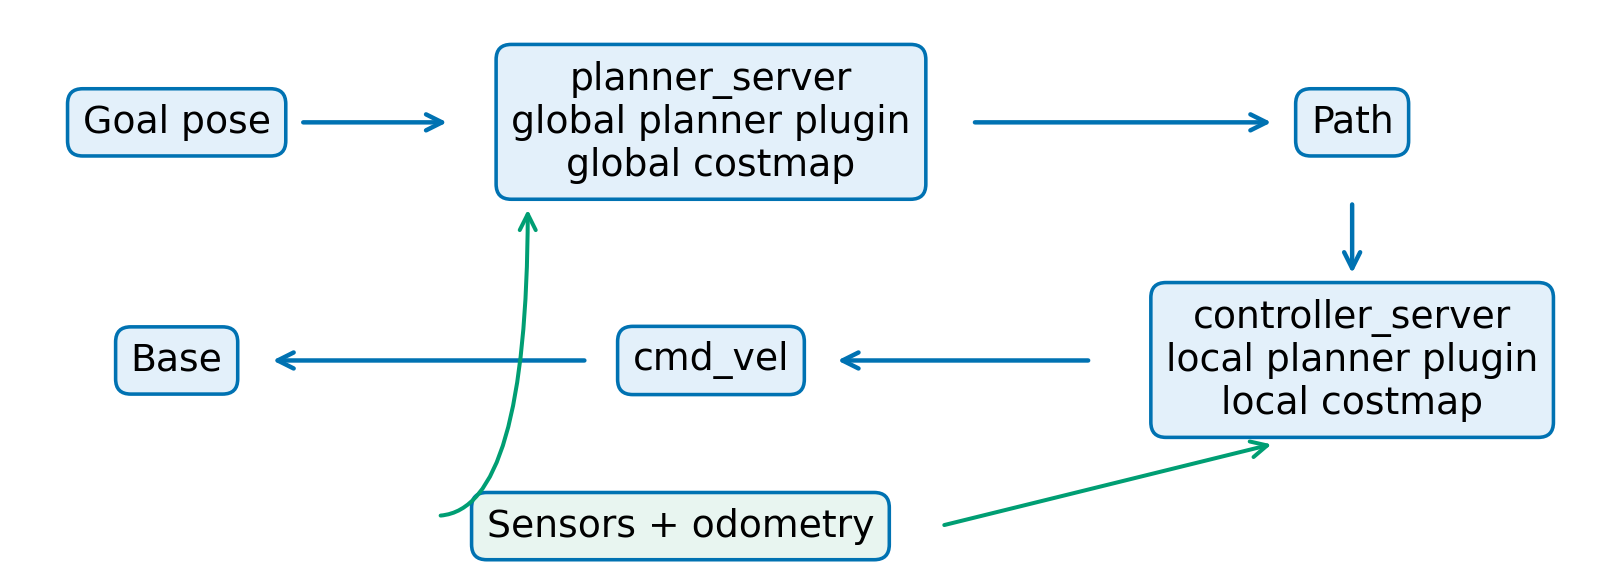
\includegraphics[width=\linewidth,height=4.5cm,keepaspectratio]{nav2_pipeline.png}\par}\textbf{Plugin}: a replaceable algorithm loaded by name. Default controller: 20 Hz.\par\href{https://github.com/ros-navigation/navigation2}{ros-navigation/navigation2}: ROS 2 navigation stack. {\scriptsize Repository defaults; check your release.}
\end{frame}

\begin{frame}[t]{Global planner: search on a costmap}
\small
\setlength{\abovedisplayskip}{1mm}\setlength{\belowdisplayskip}{1mm}
{\centering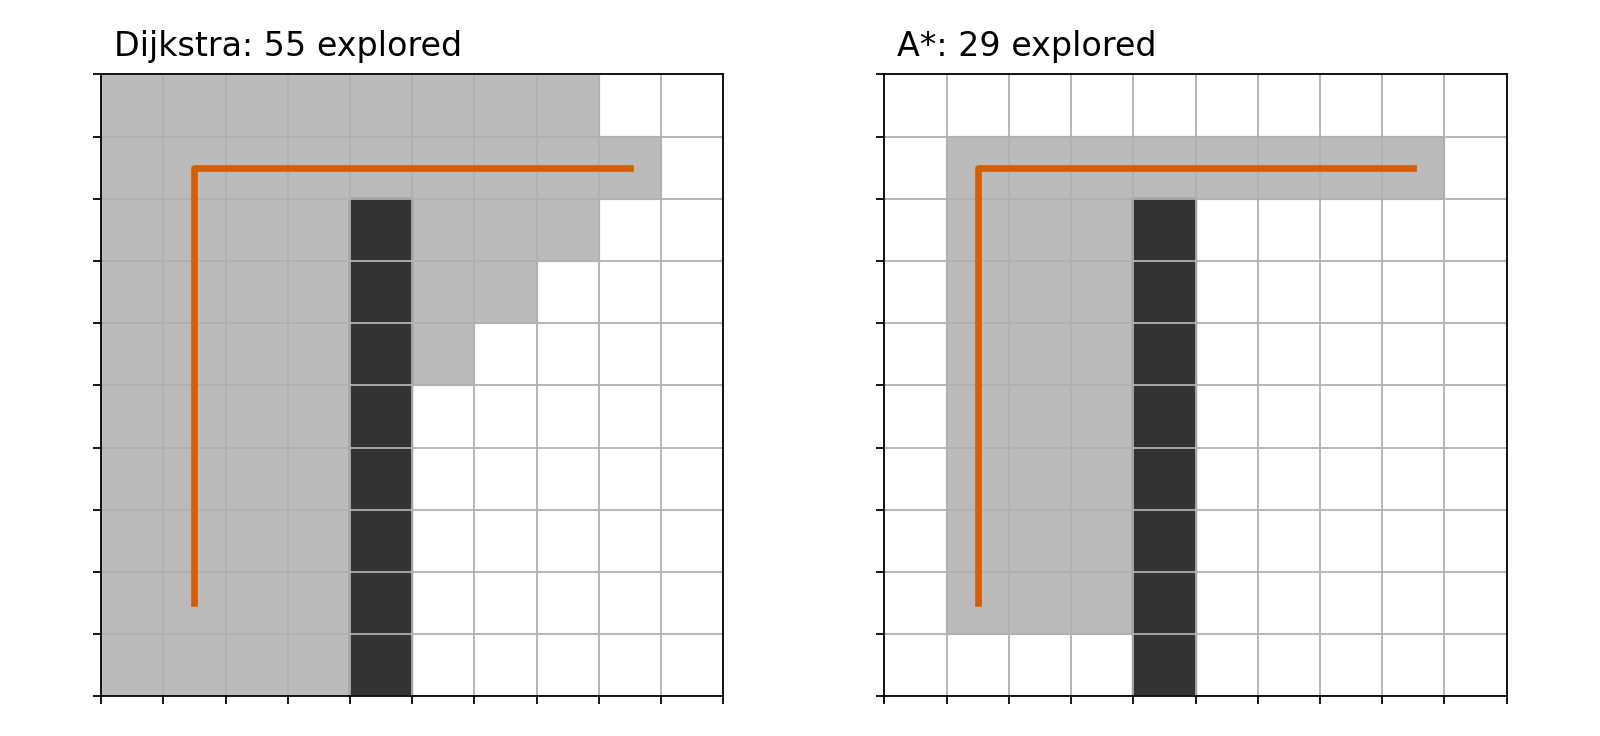
\includegraphics[width=\linewidth,height=4.5cm,keepaspectratio]{grid_search.png}\par}Costmap: danger grid. Input: costmap, start, goal; output: a path of poses.\par Dijkstra expands outward; A* uses a heuristic (estimated goal distance) to focus the search.\par NavFn: circular robot; default Dijkstra (\texttt{use\_astar=false}). {\scriptsize Repository defaults; check your release.}
\end{frame}

\begin{frame}[t]{Global planners that respect kinematics}
\small
\setlength{\abovedisplayskip}{1mm}\setlength{\belowdisplayskip}{1mm}
\vspace{-3mm}
{\centering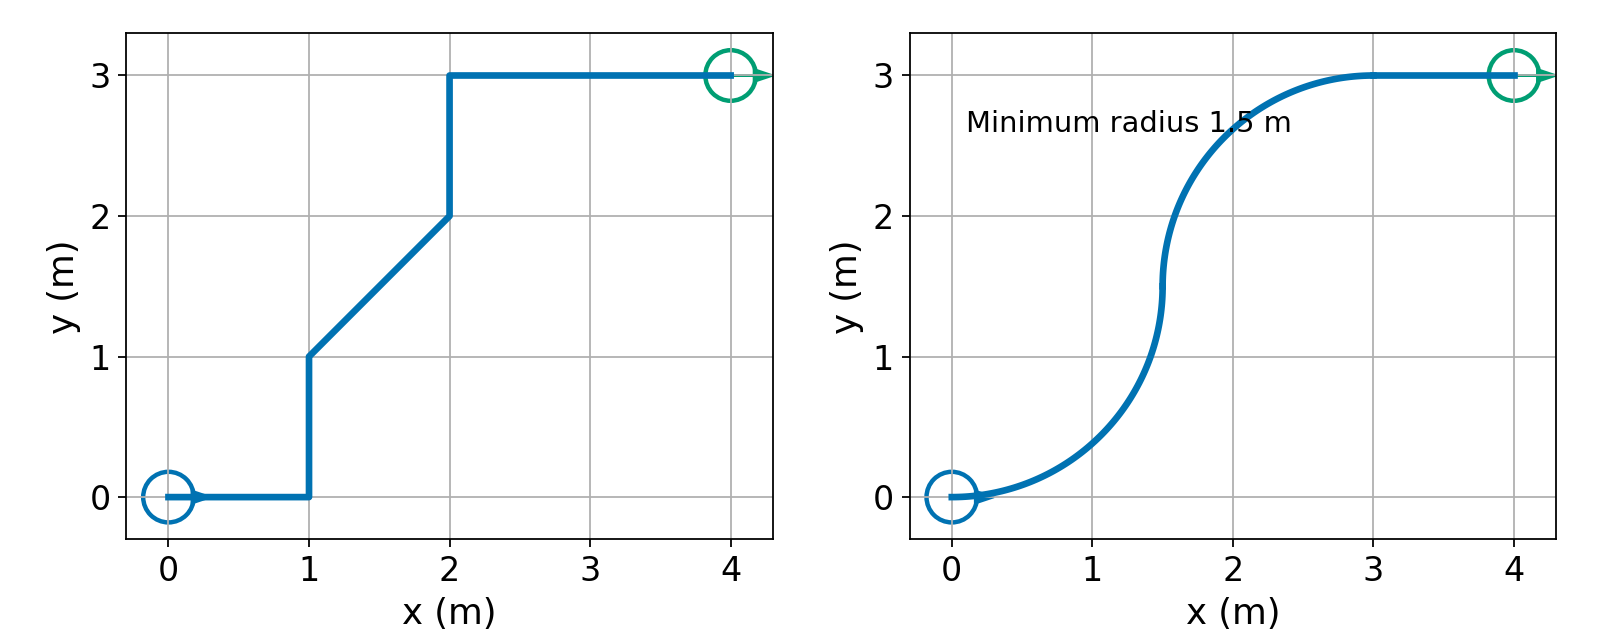
\includegraphics[width=\linewidth,height=4.5cm,keepaspectratio]{hybrid_astar.png}\par}\begin{columns}[T,onlytextwidth]\begin{column}{.49\textwidth}Smac 2D: 8-connected grid A* for circular diff./omni.\par Hybrid-A*: Dubins/Reeds--Shepp, minimum radius.\end{column}\begin{column}{.49\textwidth}Lattice: primitives for diff., omni, legged, Ackermann; any footprint. Feasible search uses actual heading.\par\href{https://github.com/ros-navigation/navigation2/tree/main/nav2_smac_planner}{Smac package}. Illustration, not Nav2 output.\end{column}\end{columns}
\end{frame}

\begin{frame}[t]{Local planner: follow the path now, avoid what is near}
\small
\setlength{\abovedisplayskip}{1mm}\setlength{\belowdisplayskip}{1mm}
\setlength{\abovedisplayshortskip}{0pt}\setlength{\belowdisplayshortskip}{0pt}
\begin{block}{Inputs and output at every control tick}
Path + local costmap + odometry $\longrightarrow$ velocity command $(v,\omega)$. The controller server repeats at 20 Hz by default.
\end{block}\vspace{2mm}
\begin{columns}[T,onlytextwidth]\begin{column}{0.49\textwidth}
\begin{block}{Path trackers}
Pure pursuit aims at a point on the path. RPP slows near obstacles and sharp curves. README: over 1 kHz on a modern CPU.
\end{block}\vspace{2mm}
\href{https://github.com/ros-navigation/navigation2/tree/main/nav2_regulated_pure_pursuit_controller}{Regulated Pure Pursuit}\end{column}\begin{column}{0.49\textwidth}
\begin{block}{Sampling planners}
DWB and MPPI simulate candidate motions, score them and choose a command.
\end{block}\vspace{2mm}
\href{https://github.com/ros-navigation/navigation2/tree/main/nav2_dwb_controller}{DWB}\quad \href{https://github.com/ros-navigation/navigation2/tree/main/nav2_mppi_controller}{MPPI}\end{column}\end{columns}\par\vspace{1mm}{\scriptsize Defaults in the Nav2 repository; check your release.}
\end{frame}

\begin{frame}[t]{Global versus local: the table}
\small
\setlength{\abovedisplayskip}{1mm}\setlength{\belowdisplayskip}{1mm}
\setlength{\abovedisplayshortskip}{0pt}\setlength{\belowdisplayshortskip}{0pt}
\renewcommand{\arraystretch}{1.1}\begin{tabularx}{\linewidth}{lXX}
\toprule Property & Global planner & Local controller\\\midrule
Role & where to go & how to move now\\
Looks at & whole known map & nearby costmap + odometry\\
Horizon & whole route & a few seconds\\
Runs & new goal / replanning trigger & every tick (default 20 Hz)\\
Kinematics & approximate, or feasible model & configured motion model\\
Failure & no route / stale map & stuck / oscillation / collision\\
Examples & NavFn, Smac & DWB, MPPI, RPP\\\bottomrule\end{tabularx}
\par\vspace{1mm}{\scriptsize Defaults in the Nav2 repository; check your release.}
\end{frame}

\begin{frame}[t]{Costmap and inflation}
\small
\setlength{\abovedisplayskip}{1mm}\setlength{\belowdisplayskip}{1mm}
\setlength{\abovedisplayshortskip}{0pt}\setlength{\belowdisplayshortskip}{0pt}
\begin{columns}[T,onlytextwidth]\begin{column}{0.49\textwidth}
\centering\begin{tikzpicture}[scale=.65]\draw[step=1,gray!30] (0,0) grid (7,6);\fill[orange!15](3,3) circle (2);\fill[orange!35](3,3) circle (1.3);\fill[black](2.5,2.5) rectangle (3.5,3.5);\draw[blue,thick](5.5,2) circle (.5);\node at (3,-.5){Obstacle, inflation halo, robot circle};\end{tikzpicture}\end{column}\begin{column}{0.49\textwidth}
\begin{block}{One cost per cell}
Values range from free to lethal. \textbf{Inflation} spreads obstacle cost outward. Point-cost critics need obstacles expanded by the robot radius, so collision can be assessed at the robot centre.
\end{block}\vspace{2mm}
The global costmap covers the known map. The local costmap is a window around the robot.\vspace{2mm}\par Both planners read costmaps; they use them over different distances and times.\end{column}\end{columns}
\end{frame}

\begin{frame}[t]{Path trackers: from pure pursuit\\to Regulated Pure Pursuit}
\small
\setlength{\abovedisplayskip}{1mm}\setlength{\belowdisplayskip}{1mm}
\setlength{\abovedisplayshortskip}{0pt}\setlength{\belowdisplayshortskip}{0pt}
\begin{columns}[T,onlytextwidth]\begin{column}{0.49\textwidth}
\centering\begin{tikzpicture}[scale=.8]\draw[green!60!black,thick] (0,0)..controls(2,0)and(2,3)..(5,3);\draw[blue,thick,->](0,0)..controls(2,0)and(3,1)..(3,2.4);\fill[orange](3,2.4) circle (.12);\draw[dashed](0,0)--(3,2.4);\draw[blue](0,0) circle (.25);\node at (2.7,-.7){Lookahead point and approach arc};\end{tikzpicture}\end{column}\begin{column}{0.49\textwidth}
\textbf{Pure pursuit}\par Pick a lookahead point on the path; drive an arc toward it. Lookahead distance replaces the three gains, and a path replaces the single goal.\par\vspace{3mm}
RPP regulates speed near obstacles and sharp curves, and adapts lookahead by speed. Suitable for differential, legged and Ackermann; no omni lateral motion.\par\vspace{3mm}
\href{https://github.com/ros-navigation/navigation2/tree/main/nav2_regulated_pure_pursuit_controller}{RPP package} and \href{https://arxiv.org/abs/2305.20026}{2023 paper}. README: over 1 kHz on a modern CPU.
\end{column}\end{columns}
\end{frame}

\begin{frame}[t]{DWB: try velocities, simulate, score}
\small
\setlength{\abovedisplayskip}{1mm}\setlength{\belowdisplayskip}{1mm}
\vspace{-3mm}
{\centering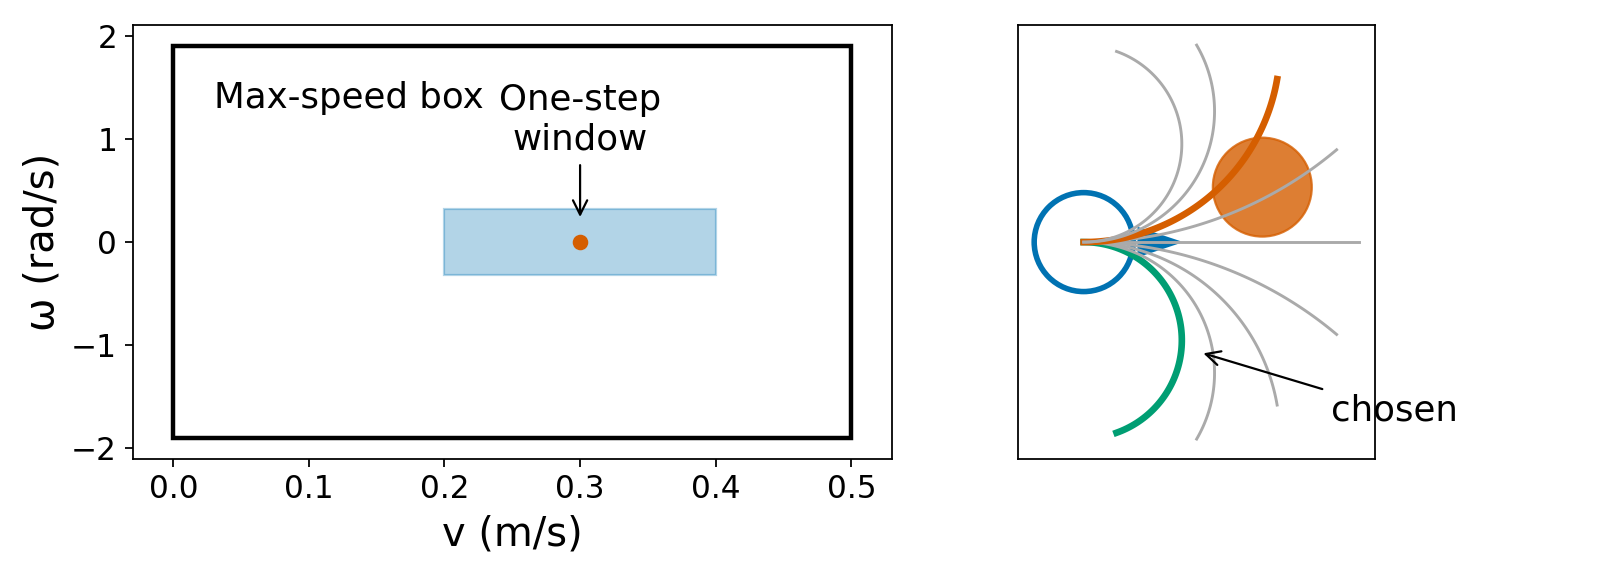
\includegraphics[width=\linewidth,height=4.5cm,keepaspectratio]{dwa_window.png}\par}\begin{columns}[T,onlytextwidth]\begin{column}{.49\textwidth}1. DWA / LimitedAccelGenerator: one-step acceleration window.\par 2. Sample $(v,\omega)$; default $20\times20$.\end{column}\begin{column}{.49\textwidth}3. Simulate constant commands: default 1.7 s.\par 4. Critic: one scoring function. Select best valid sum.\end{column}\end{columns}\vspace{1mm}\par DWB default: StandardTrajectoryGenerator (rollout style). {\scriptsize Defaults: check your release.}
\end{frame}

\begin{frame}[t]{DWB critics and tuning intuition}
\small
\setlength{\abovedisplayskip}{1mm}\setlength{\belowdisplayskip}{1mm}
\setlength{\abovedisplayshortskip}{0pt}\setlength{\belowdisplayshortskip}{0pt}
\renewcommand{\arraystretch}{1.1}\begin{tabularx}{\linewidth}{lXX}
\toprule Critic & Wants & Too much weight: intuition\\\midrule
BaseObstacle & low costmap cost & stalls in corridors\\
PathAlign / PathDist & stay on path & refuses detours\\
GoalAlign / GoalDist & head to goal & cuts corners\\
RotateToGoal & rotate at goal & creeps\\
PreferForward & forward motion & escape is harder\\
Oscillation & no back-and-forth & discourages reversals\\
Twirling & no spinning (omni) & discourages rotation\\\bottomrule\end{tabularx}
\vspace{2mm}\par \textbf{Intuition:} longer \texttt{sim\_time} sees farther, costs more compute and can slow reaction. Critic scales set priorities; collisions stay invalid.
\end{frame}

\begin{frame}[t]{MPPI: sample sequences, weight them, average}
\small
\setlength{\abovedisplayskip}{1mm}\setlength{\belowdisplayskip}{1mm}
{\centering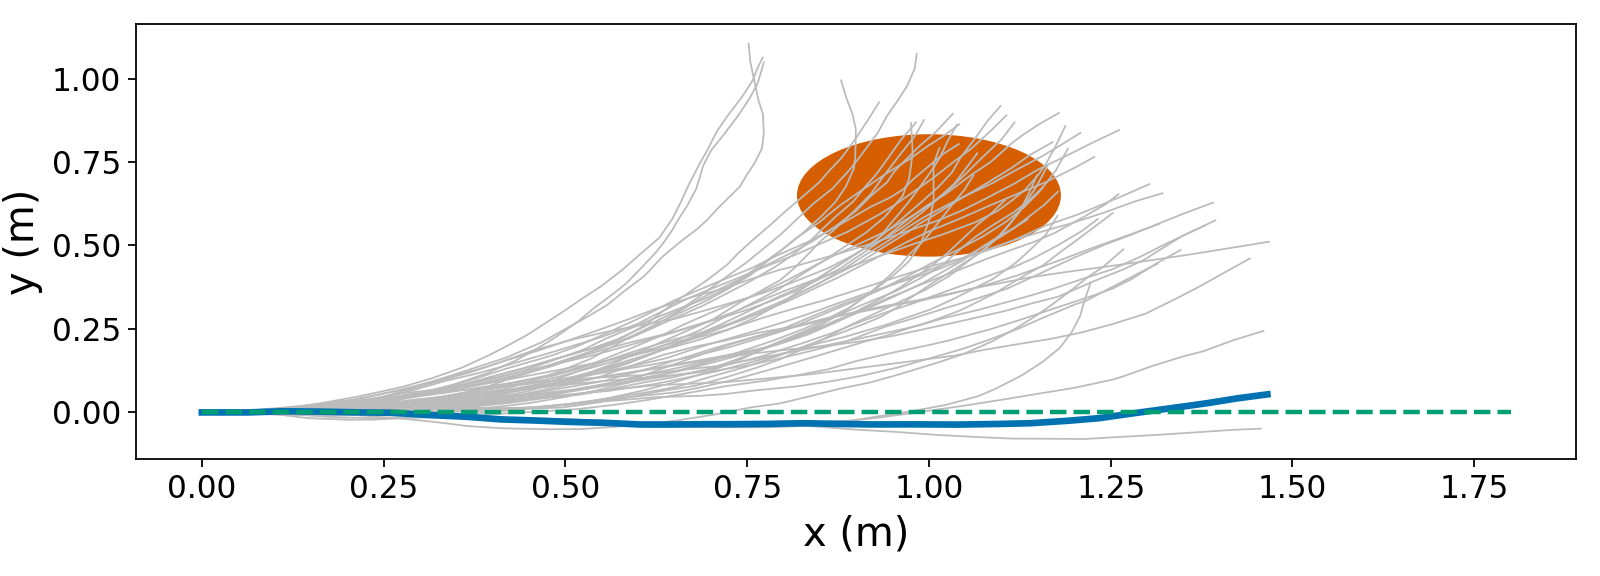
\includegraphics[width=\linewidth,height=4.5cm,keepaspectratio]{mppi_rollouts.png}\par}\begin{columns}[T,onlytextwidth]\begin{column}{.49\textwidth}1. Shift the last best control sequence.\par 2. Add Gaussian noise to make a batch.\par 3. Simulate: diff., omni or Ackermann.\end{column}\begin{column}{.49\textwidth}4. Score with critics.\par 5. Soft-max weights combine controls, not paths.\par 6. Apply first control; repeat. \href{https://github.com/ros-navigation/navigation2/tree/main/nav2_mppi_controller}{MPPI package}.\end{column}\end{columns}\par Temperature: low is selective; high approaches a plain mean of control sequences.
\end{frame}

\begin{frame}[t]{MPPI parameters and tuning intuition}
\small
\setlength{\abovedisplayskip}{1mm}\setlength{\belowdisplayskip}{1mm}

\setlength{\abovedisplayskip}{1mm}\setlength{\belowdisplayskip}{1mm}
\setlength{\abovedisplayshortskip}{0pt}\setlength{\belowdisplayshortskip}{0pt}
\renewcommand{\arraystretch}{1.0}\begin{tabularx}{\linewidth}{lXX}
\toprule Parameter & Default & Turn up: intuition\\\midrule
\texttt{time\_steps} $\times$ \texttt{model\_dt} & $56\times0.05=2.8$ s & farther, more compute\\
\texttt{batch\_size} & 1000; bringup 2000 & more candidates, CPU\\
\texttt{temperature} & 0.3 & less selective weights\\
\texttt{vx\_std}, \texttt{wz\_std} & 0.2, 0.4 & wider perturbations\\
\texttt{vx\_max}, \texttt{wz\_max} & 0.5 m/s, 1.9 rad/s & faster permitted motion\\
\texttt{gamma} & 0.015 & smoothness vs low energy\\
Critic weights & PathAlign 14; Goal 5; PreferForward 5; Cost 3.81 & greater relative priority\\\bottomrule\end{tabularx}
\vspace{2mm}\par $2.8$ s at $0.5$ m/s: $1.4$ m lookahead. Visualization slows it down.\par\vspace{1mm}{\scriptsize Defaults in the Nav2 repository; check your release.}

\end{frame}

\begin{frame}[t]{DWB versus MPPI}
\small
\setlength{\abovedisplayskip}{1mm}\setlength{\belowdisplayskip}{1mm}
\setlength{\abovedisplayshortskip}{0pt}\setlength{\belowdisplayshortskip}{0pt}
\renewcommand{\arraystretch}{1.1}\begin{tabularx}{\linewidth}{lXX}
\toprule Property & DWB & MPPI\\\midrule
Samples & DWA: constant velocity pair; default generator: rollout style & noisy control sequences\\
Combination & select one candidate & soft-max weighted controls\\
Models & differential / omni generators & differential / omni / Ackermann\\
Reported speed & not established here & 50+ Hz, 4th-gen i5 README\\
Tuning & critic scales, samples, horizon & weights, noise, temperature, horizon\\
Bringup default & earlier controller & current parameter file\\\bottomrule\end{tabularx}
\vspace{2mm}\par RPP is useful when a good path needs smooth tracking. Reported performance is hardware-specific.\par\vspace{1mm}{\scriptsize Defaults in the Nav2 repository; check your release.}
\end{frame}

\begin{frame}[t]{The rotation shim: turn first, then drive}
\small
\setlength{\abovedisplayskip}{1mm}\setlength{\belowdisplayskip}{1mm}
\vspace{-3mm}
\begin{columns}[T,onlytextwidth]\begin{column}{.62\textwidth}{\centering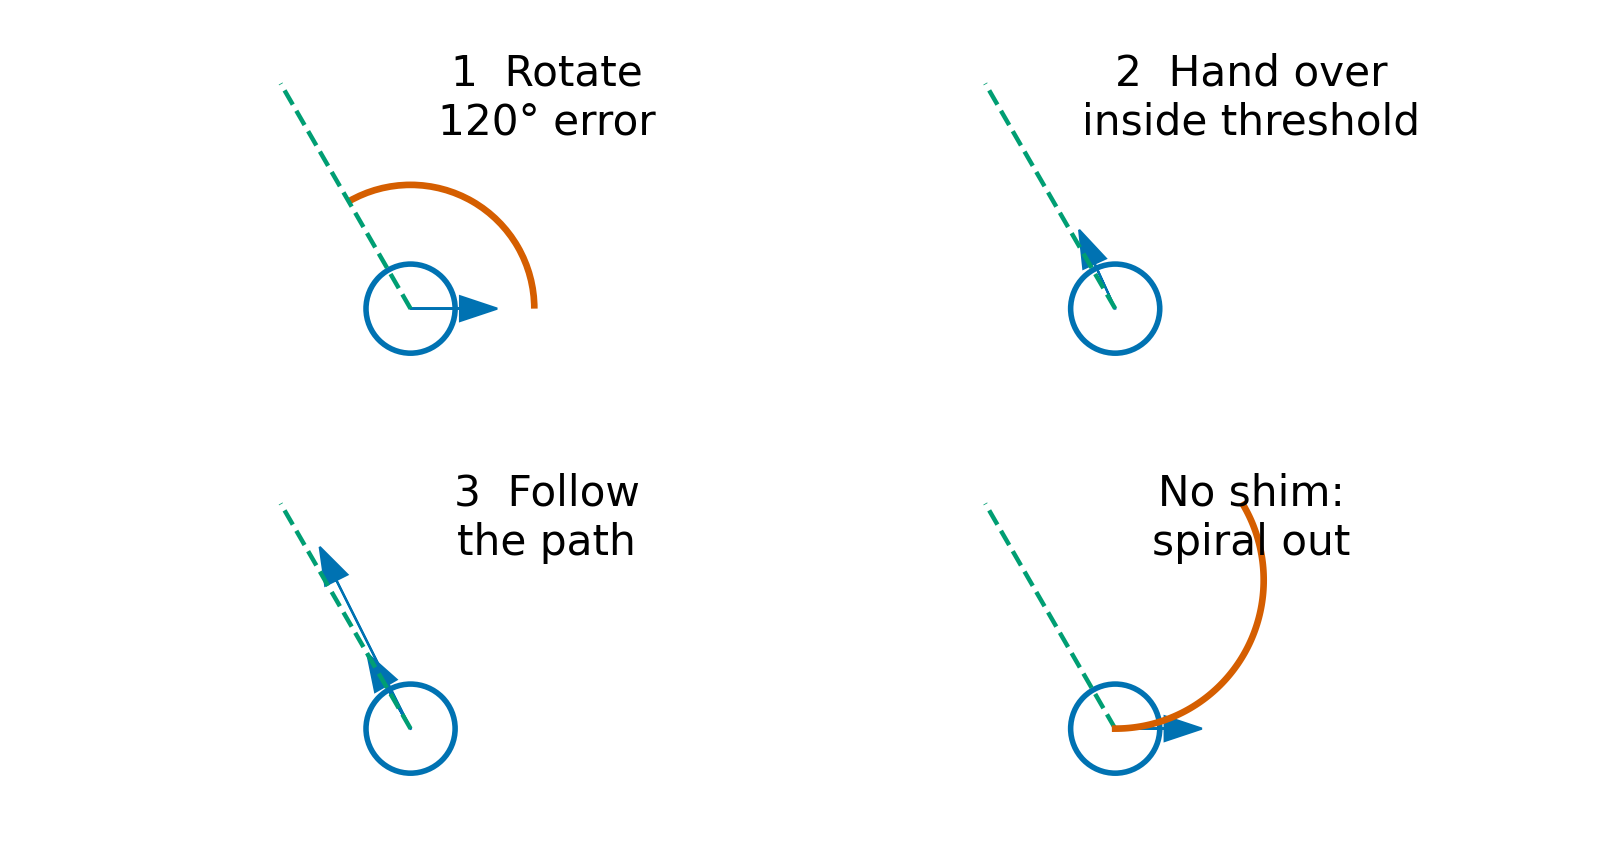
\includegraphics[width=\linewidth,height=4.5cm,keepaspectratio]{shim_sequence.png}\par}\end{column}\begin{column}{.35\textwidth}\textbf{Turn, then delegate}\par DWB/TEB can spiral out from large heading errors. The shim rotates, then delegates.\par\vspace{2mm}
Engage $0.785$ rad; hand over at $0.3925$ rad.\par Rotation $1.8$ rad/s; maximum acceleration $3.2$ rad/s$^2$.\par Heading sampled $0.5$ m ahead.\par Collision horizon $1.0$ s; return control if blocked.\par\vspace{2mm}
\href{https://github.com/ros-navigation/navigation2/tree/main/nav2_rotation_shim_controller}{Rotation shim package}.\par{\scriptsize Repository defaults; check your release.}
\end{column}\end{columns}
\end{frame}

\begin{frame}[t]{Demo 2: three controllers on the same path}
\small
\vspace{-1mm}
{\centering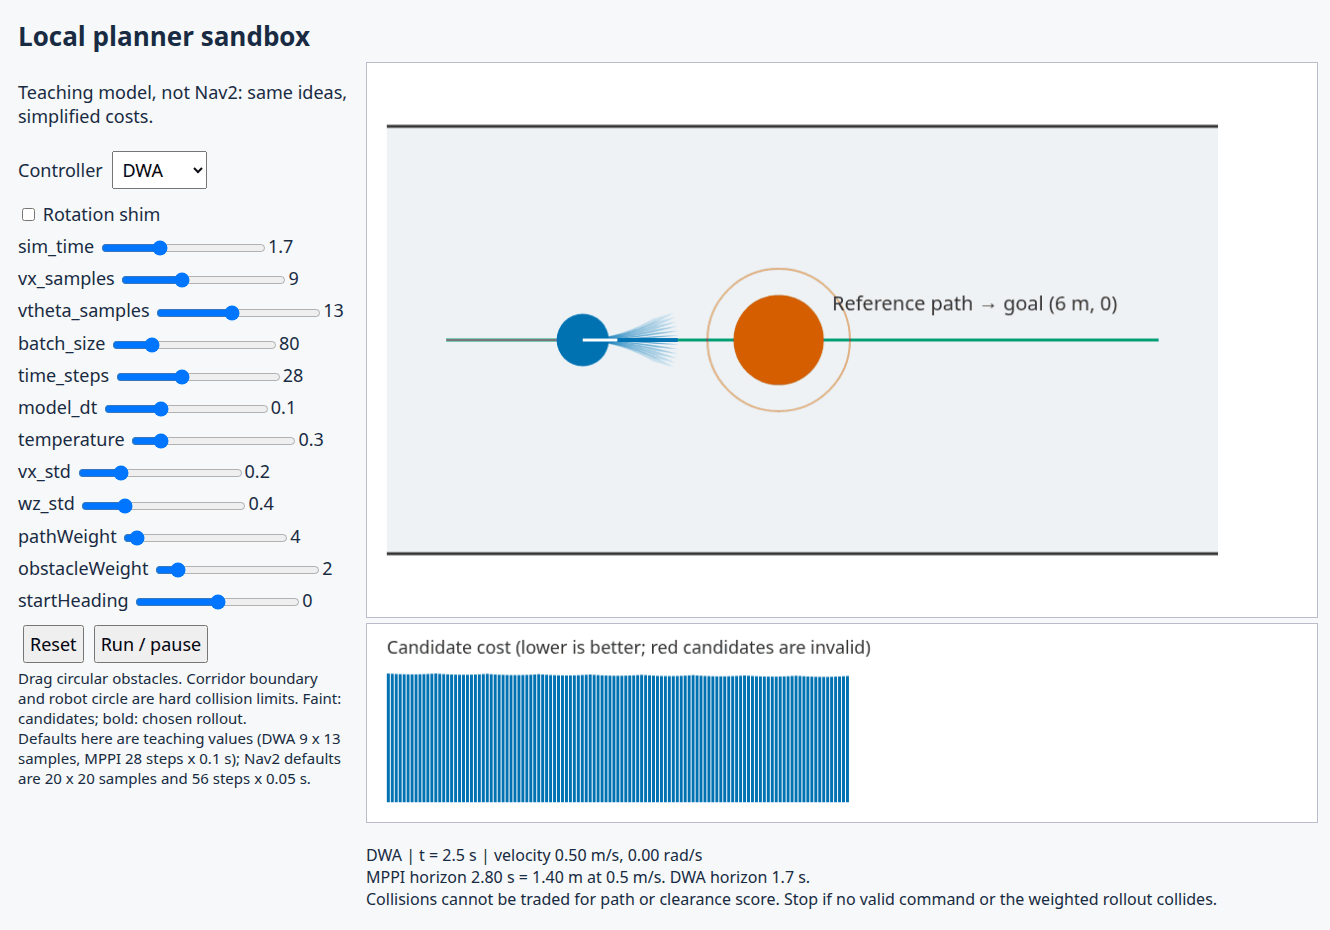
\includegraphics[width=\linewidth,height=5.5cm,keepaspectratio]{planner_demo_capture.png}\par}\textbf{Teaching model, not Nav2.} The demo uses smaller sample counts and a shorter horizon than the Nav2 defaults shown earlier.
\end{frame}

\begin{frame}[t]{Choosing a stack for a base, and what to remember}
\small
\setlength{\abovedisplayskip}{1mm}\setlength{\belowdisplayskip}{1mm}
\setlength{\abovedisplayshortskip}{0pt}\setlength{\belowdisplayshortskip}{0pt}
\renewcommand{\arraystretch}{1.05}\begin{tabularx}{\linewidth}{lXXX}
\toprule Base & Global & Local & Rotation shim\\\midrule
Differential & Smac 2D / NavFn & MPPI / DWB / RPP & with non-feasible planner\\
Omni & Smac 2D / NavFn & MPPI / DWB & useful\\
Ackermann & Hybrid / Lattice & MPPI Ackermann / RPP & no in-place rotation\\\bottomrule\end{tabularx}
\begin{block}{Five ideas to remember}
Constraints determine mobility.\par Holonomic test: DDOF $=$ DOF.\par Polar feedback: $k_\rho>0$, $k_\alpha>k_\rho$, $k_\beta<0$.\par Global: route; local: next few seconds.\par A rotation shim turns first when the base can rotate in place.
\end{block}\vspace{2mm}

\end{frame}

\begin{frame}[t]{Reference Materials}
    \begin{itemize}
        \item Siegwart, Nourbakhsh, Scaramuzza --- Siegwart Nourbakhsh Scaramuzza Introduction to Autonomous Mobile Robots Second Edition
        \item Macenski et al. --- Nav2 navigation stack, ros-navigation/navigation2
        \item Macenski, Singh, Martin, Gines --- Regulated Pure Pursuit for Robot Path Tracking
        \item Fox, Burgard, Thrun --- The dynamic window approach to collision avoidance
        \item Nav2 contributors --- MPPI controller, nav2\_mppi\_controller README
    \end{itemize}
\end{frame}


\fbckg{fibeamer/figs/last_page.png}
\frame[plain]{}

\end{document}
